% PTE Core 模考 2B —— 总整理卷（听·说·读·写 合订，自包含）
% 编译: xelatex 本文件.tex（跑两遍，目录页码才对）；依赖同目录 img/。
\documentclass[11pt]{article}

% --------- 样式（原 ptestyle.sty，已内联）---------
% ============================================================
%  ptestyle.sty  —  PTE 模考错题整理卷 共享样式
%  编译引擎: XeLaTeX  (中英混排, 需要 Noto CJK 字体)
% ============================================================

\usepackage[a4paper,margin=2cm,headsep=4mm]{geometry}
\usepackage{fontspec}
\usepackage{xeCJK}
\usepackage[table]{xcolor}
\usepackage[normalem]{ulem}        % \sout 删除线
\usepackage{tabularx}
\usepackage{array}
\usepackage{ragged2e}
\usepackage{enumitem}
\usepackage[most]{tcolorbox}
\usepackage{fancyhdr}
\usepackage{graphicx}
\usepackage{pifont}                % \ding{51}=✓ \ding{55}=✗（阅读对错标注）
\usepackage{needspace}
\usepackage{tikz}

% ---------- 字体 ----------
\setmainfont{TeX Gyre Heros}            % 拉丁: Helvetica 风格(纤细清晰)
\setCJKmainfont{Noto Sans CJK SC}
\setCJKsansfont{Noto Sans CJK SC}
\newfontfamily\cjkserif{Noto Serif CJK SC}
\linespread{1.18}
\setlength{\parindent}{0pt}
\setlength{\parskip}{4pt}

% ---------- 配色 ----------
\definecolor{cWrong}{HTML}{D32F2F}     % 红  = 修改 / 错误
\definecolor{cFix}{HTML}{1B7F3B}       % 绿  = 正确建议
\definecolor{cDelete}{HTML}{1565C0}    % 蓝  = 删除
\definecolor{cInsert}{HTML}{7B1FA2}    % 紫  = 插入
\definecolor{cPartial}{HTML}{E07B00}   % 橙  = 部分得分
\definecolor{cNote}{HTML}{0277BD}      % 蓝  = 注解
\definecolor{cAccent}{HTML}{16A085}    % 主题青绿(平台主色)
\definecolor{cWrongBg}{HTML}{FBE0E0}
\definecolor{cDelBg}{HTML}{DCE8FB}
\definecolor{cInsBg}{HTML}{EEE0F5}
\definecolor{cHead}{HTML}{20303A}
\definecolor{cGrayBox}{HTML}{F4F6F7}
\definecolor{cModelBg}{HTML}{EAF7EF}
\definecolor{cYouBg}{HTML}{FFF7F5}
\definecolor{cNoteBg}{HTML}{EAF3FA}
\definecolor{cRule}{HTML}{D7DEE2}

% ---------- 行内批改宏 (复刻平台标注) ----------
% \fix{原词}{正确}  红色删除线 + 绿色上标改正  (修改/拼写/空格)
\newcommand{\fix}[2]{%
  \colorbox{cWrongBg}{\textcolor{cWrong}{\sout{#1}}}%
  \,\textsuperscript{\textcolor{cFix}{\footnotesize #2}}}
% \del{原词}  蓝色删除线  (应删除)
\newcommand{\del}[1]{%
  \colorbox{cDelBg}{\textcolor{cDelete}{\sout{#1}}}%
  \,\textsuperscript{\textcolor{cDelete}{\footnotesize 删}}}
% \ins{词}  紫色下划线  (应插入)
\newcommand{\ins}[1]{%
  \textsuperscript{\textcolor{cInsert}{\footnotesize $\wedge$}}%
  \colorbox{cInsBg}{\textcolor{cInsert}{#1}}}
% \miss{词}  灰色删除线  (口语漏读 / 未作答)
\newcommand{\miss}[1]{\textcolor{gray}{\sout{#1}}}
% \add{原词}{改正}  橙色波浪线 + "补"标签  (平台漏标、本卷补标的错误)
\definecolor{cAdd}{HTML}{E65100}
\newcommand{\add}[2]{%
  \textcolor{cAdd}{\uwave{#1}}%
  \,\textsuperscript{\textcolor{cAdd}{\footnotesize 补：#2}}}
% 高亮(口语发音): 好/中/差
\newcommand{\spk}[2]{\textcolor{#1}{#2}}

% ---------- 评分单元格着色 ----------
\newcommand{\sfull}[1]{\textcolor{cFix}{\bfseries #1}}     % 满分
\newcommand{\spart}[1]{\textcolor{cPartial}{\bfseries #1}} % 部分
\newcommand{\szero}[1]{\textcolor{cWrong}{\bfseries #1}}   % 零/低分

% ---------- 分数小标签 ----------
\newtcbox{\chip}[1][cAccent]{on line, boxsep=2pt, left=4pt, right=4pt, top=1pt,
  bottom=1pt, arc=3pt, colback=#1, colframe=#1, coltext=white, nobeforeafter,
  fontupper=\bfseries\footnotesize}

% ---------- 题块小标题 ----------
\newcommand{\ptesub}[1]{%
  \par\needspace{2\baselineskip}\smallskip
  {\color{cAccent}\rule[-0.2ex]{3pt}{1.05em}}\hspace{6pt}%
  {\bfseries\color{cHead}#1}\par\nopagebreak\smallskip}

% ---------- 题块外框 ----------
% \begin{qblock}{标号·题型}{右上信息(得分/用时)} ... \end{qblock}
\newtcolorbox{qblock}[2]{
  breakable, enhanced, arc=2.5pt,
  colback=white, colframe=cRule, boxrule=0.6pt,
  left=11pt, right=11pt, top=8pt, bottom=10pt,
  toptitle=3pt, bottomtitle=3pt, lefttitle=11pt, righttitle=11pt,
  colbacktitle=cHead, coltitle=white, fonttitle=\bfseries,
  title={#1\hfill\normalfont\bfseries\small #2}}

% ---------- 文本块: 题干 / 范文 / 你的作答 / 建议 ----------
\newtcolorbox{promptbox}{enhanced, breakable, colback=cGrayBox, colframe=cGrayBox,
  arc=2pt, left=8pt, right=8pt, top=6pt, bottom=6pt, boxrule=0pt}
\newtcolorbox{modelbox}{enhanced, breakable, colback=cModelBg, colframe=cModelBg,
  borderline west={3pt}{0pt}{cFix}, arc=1pt, left=8pt, right=8pt, top=6pt, bottom=6pt, boxrule=0pt}
\newtcolorbox{youbox}{enhanced, breakable, colback=cYouBg, colframe=cYouBg,
  borderline west={3pt}{0pt}{cWrong}, arc=1pt, left=8pt, right=8pt, top=6pt, bottom=6pt, boxrule=0pt}
\newtcolorbox{notebox}{enhanced, breakable, colback=cNoteBg, colframe=cNoteBg,
  borderline west={3pt}{0pt}{cNote}, arc=1pt, left=8pt, right=8pt, top=6pt, bottom=6pt, boxrule=0pt}

% ---------- 评分表 ----------
% 用法见正文; 这里给表头宏
\newcommand{\scorehead}{%
  \rowcolors{2}{cGrayBox}{white}
  \arrayrulecolor{cRule}}

% ---------- 章节大标题 ----------
\newcommand{\ptesection}[3]{% #1=中文名 #2=英文名 #3=该项分数
  \addcontentsline{toc}{section}{#1}%
  \needspace{6\baselineskip}
  \begin{tcolorbox}[enhanced, colback=cAccent, colframe=cAccent, sharp corners,
     left=14pt, right=14pt, top=10pt, bottom=10pt, boxrule=0pt]
    {\fontsize{20}{24}\selectfont\bfseries\color{white} #1\ \ }%
    {\large\color{white!85} #2}\hfill
    {\large\color{white}本项得分\ \ }{\fontsize{22}{24}\selectfont\bfseries\color{white} #3}%
    \ {\color{white!85}/ 90}
  \end{tcolorbox}}

% ---------- 题型小节分隔 (口语 RA/RS/DI/RTS/ASQ 等) ----------
\newcommand{\ptetask}[2]{%
  \addcontentsline{toc}{subsection}{#1\ #2}%
  \needspace{4\baselineskip}\medskip
  \begin{tcolorbox}[enhanced, colback=cHead, colframe=cHead, sharp corners,
     left=12pt, right=12pt, top=5pt, bottom=5pt, boxrule=0pt]
    {\large\bfseries\color{white} #1}\ \ {\color{white!80} #2}
  \end{tcolorbox}\smallskip}

% ---------- 口语 AI 语音识别着色 (复刻平台: 优/良/差 + 停顿) ----------
\definecolor{cSpkGood}{HTML}{2E9E5B}   % 优 绿
\definecolor{cSpkOk}{HTML}{C77F00}     % 良 黄/琥珀
\definecolor{cSpkBad}{HTML}{E0352B}    % 差 红
\newcommand{\sg}[1]{\textcolor{cSpkGood}{#1}}   % 优
\newcommand{\sy}[1]{\textcolor{cSpkOk}{#1}}     % 良
\newcommand{\sr}[1]{\textcolor{cSpkBad}{#1}}    % 差
\newcommand{\smiss}[1]{\textcolor{cSpkBad}{\sout{#1}}}  % 漏读 (红删除线)
\newcommand{\pse}{{\color{gray}\,/\,}}          % 停顿
\newcommand{\asrlegend}{{\footnotesize\color{gray}AI 语音识别\quad
  {\color{cSpkGood}\textbullet}\,优\ \ {\color{cSpkOk}\textbullet}\,良\ \
  {\color{cSpkBad}\textbullet}\,差\ \ {\color{gray}/}\,停顿\ \
  {\color{cSpkBad}\sout{词}}\,漏读}}
\newtcolorbox{asrbox}{enhanced, breakable, colback=white, colframe=cRule,
  boxrule=0.6pt, arc=1pt, left=8pt, right=8pt, top=6pt, bottom=6pt}

% ---------- 中文翻译行 ----------
\newcommand{\zh}[1]{{\footnotesize\textcolor{cNote}{\textbf{译}}\ \textcolor{gray}{#1}}}

% ---------- 阅读填空 / 选择 对错标注 ----------
\newcommand{\rok}[1]{{\color{cFix}\ding{51}\,#1}}                 % 选对(绿勾 + 词)
\newcommand{\rno}[2]{{\color{cWrong}\ding{55}\,\sout{#1}}\,{\footnotesize\color{cFix}(答案:\,#2)}}  % 选错: 你的(红删) + (答案:正确)
\newcommand{\rblank}[1]{{\color{cFix}\underline{\,#1\,}}}         % 直接给空的正确答案(无你的作答时)

% ---------- 听力专用 ----------
\newcommand{\hiw}[2]{{\color{cWrong}\uline{#1}}\,{\footnotesize\color{cFix}(听:#2)}} % HIW: 屏幕错词(红下划线)+ 实际读音
\newcommand{\lhit}[1]{{\color{cFix}#1}}                           % WFD: 命中的词(绿)
\newcommand{\lmiss}[1]{{\color{cWrong}\sout{#1}}}                 % WFD: 多余/错误的词(红删, 1B 配色)
% ---- WFD 逐词批改 · 本套 2B 平台配色（与 1B 相反）：绿=命中 / 红括号=漏写 / 灰删除线=多写或听错 ----
% 说明: 2B 平台把"漏写"标红(加括号)、"多写/听错"标灰删除线; 本卷忠于原图按此复刻。
\newcommand{\womit}[1]{{\color{cWrong}(#1)}}                      % WFD: 漏写(正确答案有、你没写)——红色括号
\newcommand{\wbad}[1]{{\color{gray}\sout{#1}}}                    % WFD: 多写/听错(你写了但错)——灰删除线
\newcommand{\wfdlegend}{{\footnotesize\color{gray}WFD 配色：\
  {\color{cFix}命中}\ \ {\color{cWrong}(漏写)}\ \ {\color{gray}\sout{多写/听错}}}}

% ---------- 颜色图例 ----------
\newcommand{\ptelegend}{%
  \begin{tcolorbox}[enhanced, colback=cGrayBox, colframe=cRule, boxrule=0.5pt,
    arc=2pt, left=10pt, right=10pt, top=6pt, bottom=6pt]
  {\bfseries\color{cHead}颜色说明\quad}
  \fix{改}{正}~修改/拼写\quad
  \del{删}~应删除\quad
  \ins{插}~应插入\quad
  \add{补}{改正}~平台漏标(本卷补标)\quad
  {\color{cFix}\rule{1em}{0.6em}}~范文/正确\quad
  {\color{cNote}\rule{1em}{0.6em}}~AI 建议
  \end{tcolorbox}}

% ---------- 页眉页脚 ----------
\pagestyle{fancy}
\fancyhf{}
\renewcommand{\headrulewidth}{0.4pt}
\renewcommand{\footrulewidth}{0pt}
\fancyhead[L]{\footnotesize\color{cHead}\bfseries PTE Core 模考 2B}
\fancyhead[R]{\footnotesize\color{gray} 错题与详解整理卷}
\fancyfoot[C]{\footnotesize\color{gray}\thepage}
\renewcommand{\contentsname}{目录\quad Contents}

\begin{document}

% --------- 封面（原 cover.tex）---------
% ---------- 封面 / 成绩总览 ----------
\definecolor{mListen}{HTML}{1F3A5F}
\definecolor{mRead}{HTML}{C2D70B}
\definecolor{mSpeak}{HTML}{4D4D4D}
\definecolor{mWrite}{HTML}{A01B7D}

\begin{titlepage}
\thispagestyle{empty}
\centering
\vspace*{1.4cm}

{\fontsize{30}{36}\selectfont\bfseries\color{cHead} PTE Core 模考 2B}\\[4mm]
{\fontsize{17}{20}\selectfont\color{cAccent}\bfseries 错题与详解 · 整理卷}\\[3mm]
{\color{gray} APEUni / 猩际 PTE 模考　·　提交时间 2026-06-28 11:49}\\[1.2cm]

% ---- 总分 ----
\begin{tcolorbox}[width=0.62\textwidth, halign=center, enhanced,
  colback=cAccent, colframe=cAccent, arc=6pt, boxrule=0pt, top=10pt, bottom=10pt]
  {\color{white}\large 总分 Overall}\\[2pt]
  {\fontsize{46}{50}\selectfont\bfseries\color{white} 50}
\end{tcolorbox}

\vspace{1.0cm}

% ---- 四项分数条形图 ----
\begin{tcolorbox}[width=0.84\textwidth, enhanced, colback=white, colframe=cRule,
  boxrule=0.8pt, arc=4pt, left=18pt, right=18pt, top=14pt, bottom=14pt]
\setlength{\tabcolsep}{6pt}\renewcommand{\arraystretch}{1.7}
\sffamily
\begin{tabular}{@{}r@{\hskip 8pt}l@{\hskip 10pt}l@{}}
 \bfseries Listening 听力 & {\color{mListen}\rule{5.22cm}{0.42cm}} & {\bfseries\large 47}\\
 \bfseries Reading 阅读   & {\color{mRead}\rule{5.11cm}{0.42cm}}   & {\bfseries\large 46}\\
 \bfseries Speaking 口语  & {\color{mSpeak}\rule{4.00cm}{0.42cm}}  & {\bfseries\large 36}\\
 \bfseries Writing 写作   & {\color{mWrite}\rule{7.89cm}{0.42cm}}  & {\bfseries\large 71}\\
\end{tabular}\\[2mm]
{\footnotesize\color{gray} 满分 90　|　刻度: 条长 = 得分 / 90}
\end{tcolorbox}

\vfill
\begin{flushleft}\small\color{gray}
\textbf{说明:}本卷由本次模考的题目与"详解"截图逐题誊写、重新排版而成,完整保留每道题的
\emph{题干 / 原文、范文、你的作答、逐项评分、彩色批改与 AI 中文建议}。\\
所有错误按平台标注用颜色标出(见下方图例)。原始"详解"PDF 不可复制、仅截图,本卷内容均为人工对照誊录,若与原图有出入以原图为准。
\end{flushleft}
\vspace{4mm}
\ptelegend
\end{titlepage}

% --------- 目录 + 本卷概览 ---------
\clearpage
\tableofcontents
\bigskip

{\large\bfseries\color{cAccent}本卷概览}\par\smallskip
{\small
\begin{tabularx}{\linewidth}{@{}l c >{\RaggedRight\arraybackslash}X r@{}}
\rowcolor{cHead}\textcolor{white}{\bfseries 部分} & \textcolor{white}{\bfseries 题量} & \textcolor{white}{\bfseries 题型构成} & \textcolor{white}{\bfseries 本项得分}\\
听力 Listening & 15 & SST · MCM-L · FIB-L\,$\times$3 · MCS-L · SMW\,$\times$2 · HIW\,$\times$3 · WFD\,$\times$4 & 47 / 90\\
口语 Speaking & 30 & RA\,$\times$7 · RS\,$\times$11 · DI\,$\times$3 · RTS\,$\times$3 · ASQ\,$\times$6 & 36 / 90\\
阅读 Reading & 16 & FIB\,$\times$5 · MCM\,$\times$2 · RO\,$\times$2 · FIB(R)\,$\times$5 · MCS\,$\times$2 & 46 / 90\\
写作 Writing & \phantom{0}4 & SWT\,$\times$2 · WE\,$\times$2 & 71 / 90\\
\end{tabularx}}
\par\smallskip
{\footnotesize\color{gray}总分 50（听力 47 / 阅读 46 / 口语 36 / 写作 71）。颜色与标注沿用各部分；本合订本顺序为「听·说·读·写」。}

\clearpage
% --------- 四部分正文 ---------
% ===== sec_listening_body.tex =====
% ===================== 听力 Listening =====================
\ptesection{听力}{Listening · 7 题型}{47}

\vspace{1mm}
{\small\color{gray} 本部分共 \textbf{15 题}：\textbf{SST 概述口语}Q1、\textbf{MCM-L 多选}Q2、\textbf{FIB-L 听力填空（打字）}Q3--5、\textbf{MCS-L 单选}Q6、\textbf{SMW 选词}Q7--8、\textbf{HIW 找错词}Q9--11、\textbf{WFD 听写句子}Q12--15。每题保留\textbf{录音原文}（听力口语稿，含口误照原样誊录）、你的作答与平台评分，并附\textbf{中文翻译}。
标注约定：FIB-L 空处 \rok{绿勾}=对、{\color{cWrong}\ding{55}}\,红叉=错并给答案；HIW 屏幕错词用{\color{cWrong}\uline{红下划线}}标出并括注\,{\footnotesize\color{cFix}(听:实际读音)}；WFD 逐词批改本套 2B 配色为 \wfdlegend 。
本套听力总分 \textbf{47 / 90}。}
\vspace{1mm}

{\small\color{gray}\textbf{说明：}SST 的\textbf{录音原文}复盘截图未提供（需在平台「查看原题」复制），本版本（000）暂缺并标注；其余题型的录音 Transcript 复盘页均直接给出，已照抄。}
\vspace{2mm}

\newcolumntype{Z}{>{\RaggedRight\arraybackslash}X}

% ---------------- Q1 ----------------
\begin{qblock}{Q1\quad SST (C) \#5\ \ Preserving Biodiversity}{概述口语 · 评分 \textcolor{cAccent}{\bfseries 8.9 / 10}}
\ptesub{录音原文 Transcript}
\begin{promptbox}
{\color{cWrong}（录音原文：复盘截图未提供，需在平台点本题「查看原题」复制后补入；本版本（000）暂缺。）}
\end{promptbox}
\ptesub{你的概述 Your Summary}
\begin{youbox}
In the university, we should save food and protect the \fix{environmet}{environment}. Climate change will impact human beings, and many \fix{food}{foods} like rice and so on.
\end{youbox}
\zh{在大学里，我们应当节约粮食、保护环境。气候变化将影响人类，以及许多像稻米这样的粮食等等。}
{\footnotesize\color{gray}（平台彩色标注：environmet —— 拼写错误，应为 environment；food —— 应为复数 foods。）}
\ptesub{AI 评分明细（满分 10）}
\begin{notebox}
{\renewcommand{\arraystretch}{1.35}
\begin{tabularx}{\linewidth}{@{}l c Z@{}}
\textbf{单项} & \textbf{得分} & \textbf{AI 建议}\\[2pt]
Content（内容）& \sfull{2 / 2} & 内容很棒。\\
Form（形式）& \sfull{2 / 2} & Form 很棒，这是必拿分数。\\
Grammar（语法）& \spart{1.5 / 2} & 点击有颜色标注的文字查看语法错误细节。\\
Spelling（拼写）& \sfull{2 / 2} & 虽然你拼写拿了满分，但还是犯了 1 个拼写错误，下次注意避免。\\
Vocabulary（词汇）& \spart{1.4 / 2} & PTE 对词汇不要求很难，但需要恰当。\\
\end{tabularx}}
\smallskip
\textbf{本题分值}\ 10 分\qquad\textbf{你的总得分}\ \textcolor{cAccent}{\bfseries 8.9 / 10}
\end{notebox}
\smallskip
{\footnotesize\color{gray}（答题用时 05:46；失分主要在 Grammar 与 Vocabulary。）}
\end{qblock}

% ---------------- Q2 ----------------
\begin{qblock}{Q2\quad MCM-L \#119\ \ Weight Gain}{多选 · 评分 \textcolor{cAccent}{\bfseries 2 / 2}}
\ptesub{录音原文 Transcript}
\begin{promptbox}
Both men and women gained weight but when it came to race, black women had the most rapid weight gain, followed by white women and then black and white men. The weight gain was just a few pounds---but even a slightly higher BMI is associated with weight-related health issues. Several reasons exist for the weight discrepancy between the single and married people. For example, married men and women may be less concerned about their body weight because they're no longer actively seeking a mate. Plus, married people have a regular dining partner, possibly leading to more meals. On the single side, those who are widowed or have gone through a divorce may lose weight due to stress. So while this news may not be good for the smug marrieds, it may be welcomed by Bridget Jones. The single, and very weight-conscious, Jones may actually have had the easier path to staying thin than her married friends.
\end{promptbox}
\zh{男性和女性都会增重，但就种族而言，黑人女性增重最快，其次是白人女性，再次是黑人和白人男性。增重只有几磅——但即便 BMI 略高，也与体重相关的健康问题有关。单身者与已婚者之间体重差异有几个原因。例如，已婚男女可能不太在意体重，因为他们不再积极寻找伴侣；加上已婚者有固定的用餐伙伴，可能导致进餐更多。另一方面，丧偶或离婚的单身者可能因压力而体重下降。所以这条新闻对自得的已婚者也许不是好消息，却可能受到 Bridget Jones 的欢迎——单身且非常在意体重的 Jones 也许比已婚的朋友更容易保持苗条。}
\ptesub{题目 Question}
\begin{notebox}Why are married people more likely to gain weight?\end{notebox}
\ptesub{选项 Choices（正确项绿色加粗）}
{\small
{\color{cFix}\textbf{A) Because they have regular dining partners and probably have more meals.}}\\
B) Because people's life is less stressful after marriage.\\
{\color{cFix}\textbf{C) Because they don't need to find a mate anymore and care less about their weight.}}\\
D) Because they are happier after marriage and eat more.\\
E) Because their partners require them to eat more.}
\par\smallskip
\textbf{正确答案}\ \textcolor{cFix}{\bfseries A, C}\qquad\textbf{你的答案}\ \textcolor{cFix}{\bfseries A, C}\qquad\textbf{本题得分：}\ {\color{cAccent}\bfseries 2 / 2}\quad{\footnotesize\color{gray}（用时 01:06，全对）}
\end{qblock}

% ---------------- Q3 ----------------
\begin{qblock}{Q3\quad FIB-L \#166\ \ Cultural Heritage}{听力填空（打字）· 评分 \textcolor{cAccent}{\bfseries 0 / 4}}
\ptesub{录音原文 Transcript（含填空作答）}
\begin{promptbox}
All around the world, significant parts of our cultural heritage are \rno{strenthen}{threatened} by pollution, neglect, \rno{careless}{carelessness} and greed. In learning the importance of our history, we come to understand the need to protect significant \rno{construction}{remains} from the past so that future \rno{construction}{generations} can come to understand their heritage.
\end{promptbox}
\zh{世界各地，我们文化遗产的重要部分正受到污染、忽视、疏忽大意与贪婪的威胁。在认识历史重要性的过程中，我们逐渐明白必须保护来自过去的重要遗存，好让后代也能理解他们的遗产。}
\par\smallskip
\textbf{你的作答：}\ {\color{cWrong}strenthen, careless, construction, construction}\qquad\textbf{本题得分：}\ {\color{cAccent}\bfseries 0 / 4}\quad{\footnotesize\color{gray}（用时 01:04；四空全错，正确为 threatened / carelessness / remains / generations）}
\end{qblock}

% ---------------- Q4 ----------------
\begin{qblock}{Q4\quad FIB-L \#208\ \ Well-being}{听力填空（打字）· 评分 \textcolor{cAccent}{\bfseries 1 / 3}}
\ptesub{录音原文 Transcript（含填空作答）}
\begin{promptbox}
Life in the UK 2012 provides a unique overview of well-being in the UK today. The report is the first snapshot of life in the UK to be \rno{diliver}{delivered} by the Measuring National Well-being program and will be updated and published annually. Well-being is discussed in terms of the economy, people and the environment. Information such as the \rno{unemployed}{unemployment} rate or number of crimes against the person are presented alongside data on people's thoughts and feelings, for example, \rok{satisfaction} with our jobs or leisure time and fear of crime. Together, a richer picture on `how society is doing' is provided.
\end{promptbox}
\zh{《2012 年英国生活》对当今英国的福祉作了独特的总览。该报告是首份由"国家福祉测量"项目发布的英国生活快照，并将每年更新发布。福祉从经济、民众与环境三方面来讨论。诸如失业率或针对个人的犯罪数量等信息，会与人们的想法和感受数据一并呈现，例如对工作或闲暇时间的满意度、对犯罪的担忧等。如此便提供了一幅关于"社会运行得如何"的更丰富图景。}
\par\smallskip
\textbf{你的作答：}\ {\color{cWrong}diliver}, {\color{cWrong}unemployed}, satisfaction\qquad\textbf{本题得分：}\ {\color{cAccent}\bfseries 1 / 3}\quad{\footnotesize\color{gray}（用时 01:09；仅第 3 空 satisfaction 正确，diliver→delivered、unemployed→unemployment）}
\end{qblock}

% ---------------- Q5 ----------------
\begin{qblock}{Q5\quad FIB-L \#95\ \ Oceanographer}{听力填空（打字）· 评分 \textcolor{cAccent}{\bfseries 0 / 4}}
\ptesub{录音原文 Transcript（含填空作答）}
\begin{promptbox}
For many years the favorite horror story about \rno{abrot}{abrupt} climate change was that a shift in ocean currents could \rno{directly}{radically} cool Europe's climate. These currents, called the overturning \rno{servculation}{circulation} bring warm water and warm temperatures north from the equator to Europe. Susan Loosier, an \rno{profossor}{oceanographer} at Duke University, says scientists have long worried that this ocean circulation could be disrupted.
\end{promptbox}
\zh{多年来，关于突变性气候变化最受关注的"恐怖故事"是：洋流的转变可能使欧洲气候急剧变冷。这些被称为"翻转环流"的洋流，把温暖的海水和温度从赤道向北带到欧洲。杜克大学的海洋学家 Susan Loosier 说，科学家长期担心这种海洋环流可能被打断。}
\par\smallskip
\textbf{你的作答：}\ {\color{cWrong}abrot, directly, servculation, profossor}\qquad\textbf{本题得分：}\ {\color{cAccent}\bfseries 0 / 4}\quad{\footnotesize\color{gray}（用时 01:16；四空全错，正确为 abrupt / radically / circulation / oceanographer）}
\end{qblock}

% ---------------- Q6 ----------------
\begin{qblock}{Q6\quad MCS-L \#127\ \ Autism Diagnoses}{单选 · 评分 \textcolor{cAccent}{\bfseries 0 / 1}}
\ptesub{录音原文 Transcript}
\begin{promptbox}
The first two years of a baby's life are critical for brain development. In this study, parents were given video-based tips on how best to interact with their babies according to their particular needs. By the age of three, the baby still had some developmental difficulties, but their social skills had improved, and two thirds fewer met the criteria for a diagnosis of autism spectrum disorder, compared to babies who received standard care. The research charity Autistica said the study was promising and people should not have to wait for a diagnosis for support to be provided. But the National Autistic Society said autism was not a disease that should be cured or lessened. The research team says longer term studies on more babies using the technique are now needed.
\end{promptbox}
\zh{婴儿生命的头两年对大脑发育至关重要。在这项研究中，家长得到了基于视频的指导，学习如何根据自己孩子的特定需求与之互动。到三岁时，这些婴儿仍有一些发育困难，但社交能力有所改善，符合自闭症谱系障碍诊断标准的比例比接受常规照护的婴儿少了三分之二。研究慈善机构 Autistica 表示该研究很有前景，人们不应等到确诊才获得支持。但全国自闭症协会则表示，自闭症并非一种需要治愈或减轻的疾病。研究团队称，现在需要用该方法对更多婴儿进行更长期的研究。}
\ptesub{题目 Question}
\begin{notebox}What is the attitude of the research charity Autistica with regard to their finding?\end{notebox}
\ptesub{选项 Choices（正确项绿色加粗）}
{\small
A) Negative.\\
B) Assured.\\
C) Disdainful.\\
{\color{cFix}\textbf{D) Expectant.}}}
\par\smallskip
\textbf{正确答案}\ \textcolor{cFix}{\bfseries D}\qquad\textbf{你的答案}\ {\color{cWrong}\bfseries A}\qquad\textbf{本题得分：}\ {\color{cAccent}\bfseries 0 / 1}\quad{\footnotesize\color{gray}（用时 00:59；Autistica 认为研究"有前景"，态度是期待 Expectant）}
\end{qblock}

% ---------------- Q7 ----------------
\begin{qblock}{Q7\quad SMW \#116\ \ Filtering Tools}{选词（结尾被哔替换）· 评分 \textcolor{cAccent}{\bfseries 0 / 1}}
\ptesub{录音原文 Transcript（结尾词被「哔」替换）}
\begin{promptbox}
One of the biggest surprises of the Internet is we thought when the Internet came out it would provide everyone new fundamental tools to learn about the world around them, and it would actually remove the censorship and information that we get. We basically all have our own responsibility to become our own filters. We have, and that's why it seems to me the educational system has to provide those tools those filtering tools. And that's one of the reasons why I think science is so important because of its built-in filtering tools. It recognizes that we all want to believe and as Richard Feynman said, ``The person you have to question most is yourself.'' Knowing that you want to believe when you read something that validates your beliefs, you should be skeptical of it and your beliefs and you should look out for other sources. So we have to train people that one source on the Internet is not good enough you have to search broadly to see if it's \rule[0.3ex]{1.2cm}{0.4pt}\ \textit{[beep]}.
\end{promptbox}
\zh{互联网最大的意外之一是：我们原以为互联网问世会给每个人提供了解世界的全新基础工具，并真正消除我们所获信息中的审查。基本上我们都有责任成为自己的"过滤器"。正因如此，在我看来教育体系必须提供这些过滤工具。这也是我认为科学如此重要的原因之一——它自带过滤工具：它认清我们都"想要相信"，正如理查德·费曼所说："你最需要质疑的人是你自己。"当你读到某些印证你既有信念的东西时，要意识到自己"想相信"，从而对它、对自己的信念保持怀疑，并去寻找其他来源。所以我们必须训练人们：网上单一来源并不可靠，你必须广泛检索，看看它是否经得起＿＿＿（被验证）。}
\ptesub{选项 Choices（正确项绿色加粗）}
{\small
A) skeptical\\
B) important\\
{\color{cFix}\textbf{C) validated}}}
\par\smallskip
\textbf{正确答案}\ \textcolor{cFix}{\bfseries C}\qquad\textbf{你的答案}\ {\color{cWrong}\bfseries B}\qquad\textbf{本题得分：}\ {\color{cAccent}\bfseries 0 / 1}\quad{\footnotesize\color{gray}（用时 01:06；句末应为 validated）}
\end{qblock}

% ---------------- Q8 ----------------
\begin{qblock}{Q8\quad SMW \#21\ \ Crime}{选词（结尾被哔替换）· 评分 \textcolor{cAccent}{\bfseries 1 / 1}}
\ptesub{录音原文 Transcript（结尾词组被「哔」替换）}
\begin{promptbox}
Why do we have crime? When will it all stop? IT's sad that there is so much crime in our society. It hurts so many people. Most people in the world just want to live happily and be good neighbors. Why do some people turn to crime? Money is a big reason. Many criminals pickpocket, steal, kidnap or even kill people to get money. There are many terrible crimes in the world. Perhaps the worst is ethnic cleansing. This is a crime against humanity. Many people are killed because of their color or religion. People who commit this crime really go to prison. Have you ever been a victim of crime? What do you think we need to do to reduce crime rates? Perhaps you should run \rule[0.3ex]{1.2cm}{0.4pt}\ \textit{[beep]}.
\end{promptbox}
\zh{我们为什么会有犯罪？它何时才会停止？我们的社会有这么多犯罪，令人难过，伤害了许多人。世界上大多数人只想快乐地生活、做好邻居。为什么有些人走向犯罪？金钱是一大原因。许多罪犯为了钱去扒窃、偷盗、绑架，甚至杀人。世上有许多可怕的罪行，也许最严重的是种族清洗——这是反人类罪，许多人因肤色或宗教被杀害，犯下此罪的人真的会进监狱。你曾经是犯罪的受害者吗？你认为我们需要做什么来降低犯罪率？也许你应该跑去＿＿＿（向你的政府）。}
\ptesub{选项 Choices（正确项绿色加粗）}
{\small
{\color{cFix}\textbf{A) to your government}}\\
B) to your family\\
C) to your boss\\
D) to your friends}
\par\smallskip
\textbf{正确答案}\ \textcolor{cFix}{\bfseries A}\qquad\textbf{你的答案}\ \textcolor{cFix}{\bfseries A}\qquad\textbf{本题得分：}\ {\color{cAccent}\bfseries 1 / 1}\quad{\footnotesize\color{gray}（用时 01:06，正确）}
\end{qblock}

% ---------------- Q9 ----------------
\begin{qblock}{Q9\quad HIW \#7\ \ Light}{找错词 · 评分 \textcolor{cAccent}{\bfseries 3 / 5}}
\ptesub{录音原文 Transcript（屏幕错词\,{\color{cWrong}\uline{红下划线}}\,，括注实际读音）}
\begin{promptbox}
It follows from the special theory of relativity that mass and energy are different manifestations of the same thing. Now \hiw{cleavages}{researchers} have stopped light cold --- and then brought it back to life --- or light --- in an \hiw{ribaldry}{entirely} different place. The Harvard researchers sent a light pulse into a sodium cloud cooled to about 460 degrees below zero. That's the \hiw{hypocritical}{theoretical} point where matter stops all movement. The light pulse was compressed by a factor of about 50 million at the extreme temperature, and it actually changed state --- sort of like frozen water. But it also split into two forms of matter. One stayed frozen in the sodium, while the other crawled along at just 200 meters per hour. That second form --- called a matter wave --- contains the exact information of the original light wave. And when researchers sent it into a second sodium cloud a fraction of a \hiw{freesia}{millimeter} away, the wave was converted back into light. And since fiber-optic \hiw{containers}{communications} use light, that means that someday we may be able to stop them, store them and turn them back on, just like a light switch.
\end{promptbox}
\zh{由狭义相对论可知，质量与能量是同一事物的不同表现形式。如今研究人员让光彻底"停下"——随后又让它"复活"，或者说在另一个完全不同的地方重现光。哈佛的研究人员把一束光脉冲送入冷却到约零下 460 度的钠云中，那是物质停止一切运动的理论临界点。在这一极端温度下，光脉冲被压缩了约 5000 万倍，并真的发生了相变——有点像结冰的水，还分裂成两种物质形态：一种冻结在钠中，另一种以每小时仅 200 米的速度缓慢爬行。后一种形态——称为"物质波"——精确保留了原始光波的信息。当研究人员把它送入第二团相距仅几分之一毫米的钠云时，物质波又被转换回光。既然光纤通信使用光，这意味着将来我们也许能像开关电灯一样，让光"停下、存储、再开启"。}
\par\smallskip
\textbf{答案：}\ 实际读音（Pronounced words）\ {\color{cFix}researchers, entirely, theoretical, millimeter, communications}\\
\textbf{应点错词}\ 共 \textbf{5} 个（已红下划线标出）\qquad\textbf{你点中}\ \textbf{3} 个：ribaldry, freesia, containers（均正确）\\[2pt]\textbf{本题得分：}\ {\color{cAccent}\bfseries 3 / 5}\quad{\footnotesize\color{gray}（用时 01:15；漏点 cleavages、hypocritical）}
\end{qblock}

% ---------------- Q10 ----------------
\begin{qblock}{Q10\quad HIW \#45\ \ Crop Rotation（原图标题处仅重复"HIW"）}{找错词 · 评分 \textcolor{cAccent}{\bfseries 4 / 6}}
\ptesub{录音原文 Transcript（屏幕错词\,{\color{cWrong}\uline{红下划线}}\,，括注实际读音）}
\begin{promptbox}
Crop \hiw{exploitation}{rotation} is a recognized way to keep soil and the food ecosystem healthy. Now, \hiw{licenses}{scientists} are saying that rotation could be a useful tool---in the sea. Researchers tracked a shallow-water, near-shore species used for food: sea cucumbers. They're easy to harvest and are fairly valuable. But those same attributes mean they're easy to overharvest. The \hiw{indulgence}{practice} has put some sea cucumber species at high risk of extinction, even in a relatively well-managed area, the Great Barrier Marine Park in Australia. In 2004 authorities split the Great Barrier Reef into 154 zones, where each zone was fished only once every three years. Fishers rotate through the region. In computer models, the researchers ran through dozens of \hiw{avocations}{simulations} of each zone, both before and after the divisions took place. The trials revealed that even with an identical and \hiw{snapped}{low-catch} allowance in all cases, the sea cucumbers would recover more fully under the rotation strategy than by harvesting simultaneously \hiw{couched}{throughout} the region. In fact, in trials that included rotations, the yield actually increased. The research is in the Proceedings of the National Academy of Sciences. The scientists say their results suggest that such rotation might be beneficial in these kinds of shallow marine regions around the world, particularly for species that are in high demand. Because you should not eat your seed corn. Or your seed sea cucumbers.
\end{promptbox}
\zh{作物轮作是保持土壤和食物生态系统健康的公认方法。如今科学家提出，轮作在海里也可能是有用的工具。研究人员追踪了一种近岸浅水的食用物种：海参。它们容易采捕、价值不低，但这些特点也意味着容易被过度捕捞。这种做法已使一些海参物种面临极高的灭绝风险，即便在管理相对完善的澳大利亚大堡礁海洋公园也是如此。2004 年管理部门把大堡礁划分为 154 个区，每个区每三年只捕捞一次，渔民在该区域内轮换作业。在计算机模型中，研究人员对每个区在划分前后跑了数十次模拟。试验显示：即使在所有情形下都给予相同且低捕捞量的配额，海参在轮作策略下的恢复也比在整个区域同时捕捞更充分；事实上，在包含轮作的试验中产量反而增加了。该研究发表于《美国国家科学院院刊》。科学家表示，结果说明这种轮作可能对世界各地这类浅海区域有益，尤其是对需求量高的物种。因为你不该吃掉留作种子的玉米——也别吃掉留作种源的海参。}
\par\smallskip
\textbf{答案：}\ 实际读音（Pronounced words）\ {\color{cFix}rotation, scientists, practice, simulations, low-catch, throughout}\\
\textbf{应点错词}\ 共 \textbf{6} 个（已红下划线标出）\qquad\textbf{你点中}\ \textbf{4} 个：indulgence, avocations, snapped, couched（均正确）\\[2pt]\textbf{本题得分：}\ {\color{cAccent}\bfseries 4 / 6}\quad{\footnotesize\color{gray}（用时 01:27；漏点 exploitation、licenses）}
\end{qblock}

% ---------------- Q11 ----------------
\begin{qblock}{Q11\quad HIW \#53\ \ Advertising}{找错词 · 评分 \textcolor{cAccent}{\bfseries 2 / 4}}
\ptesub{录音原文 Transcript（屏幕错词\,{\color{cWrong}\uline{红下划线}}\,，括注实际读音）}
\begin{promptbox}
Companies spend \hiw{intuitions}{billions} on advertising every year. But they're not just pushing products---they're selling their brand's ``personality,'' too. Think: Red Bull. What comes to mind? Most people say things like speed...power...hyper...extreme. Well, a pair of scientists wanted to see if the energy drink's alleged qualities would \hiw{contiguous}{influence} people's performance in a racecar video game---without sipping Red Bull. So they had 70 volunteers race cars with identical specs, but different paint jobs. Four with the logo and colors of a drink---Guinness, Tropicana, Coca-Cola or Red Bull---and one car just plain green. The drivers clocked similar times with most of the cars. But behind the wheel of the Red Bull car, they \hiw{analogously}{actually} drove more aggressively, scoring either incredibly fast race times, or their slowest---by driving recklessly and crashing. The study appears in the Journal of Consumer Psychology. Polled after the game, the players didn't realize the Red Bull image apparently \hiw{phosphoenolpyruvate}{influenced} their driving. Which suggests marketing doesn't just influence a brand's personality. It could be shaping our personalities, too, without our even knowing it.
\end{promptbox}
\zh{企业每年在广告上花费数十亿。但它们推销的不只是产品——还在推销品牌的"个性"。想想红牛，你会想到什么？多数人会说速度、力量、亢奋、极限之类。于是两位科学家想看看：在不喝红牛的情况下，这款能量饮料所宣称的特质是否会影响人们在赛车电子游戏中的表现。他们让 70 名志愿者驾驶规格相同、但涂装不同的赛车：四辆带某品牌的标志和配色——健力士、纯果乐、可口可乐或红牛——还有一辆只是纯绿色。多数车上车手用时相近，但坐进红牛车时，他们实际上开得更激进：要么跑出极快的成绩，要么因鲁莽驾驶撞车而跑出最慢成绩。该研究发表于《消费者心理学杂志》。游戏后被问及时，玩家并未意识到红牛形象明显影响了他们的驾驶。这说明营销不只塑造品牌个性，也可能在我们毫无察觉时塑造我们自己的个性。}
\par\smallskip
\textbf{答案：}\ 实际读音（Pronounced words）\ {\color{cFix}billions, influence, actually, influenced}\\
\textbf{应点错词}\ 共 \textbf{4} 个（已红下划线标出）\qquad\textbf{你点中}\ \textbf{2} 个：intuitions, analogously（均正确）\\[2pt]\textbf{本题得分：}\ {\color{cAccent}\bfseries 2 / 4}\quad{\footnotesize\color{gray}（用时 01:16；漏点 contiguous、phosphoenolpyruvate）}
\end{qblock}

% ---------------- Q12 ----------------
\begin{qblock}{Q12\quad WFD \#1973}{听写句子 · 评分 \textcolor{cAccent}{\bfseries 4 / 9}}
\ptesub{正确句子 Sentence}
\begin{promptbox}
You will acquire many skills during the academic studies.
\end{promptbox}
\zh{在学术学习期间，你将获得许多技能。}
\ptesub{你的作答（逐词批改）\quad{\normalfont\wfdlegend}}
\begin{youbox}
\lhit{you} \womit{will acquire} \wbad{are required} \lhit{many skills} \womit{during the academic} \wbad{to join in your acadamic study} \lhit{studies}
\end{youbox}
\smallskip
\textbf{本题得分：}\ {\color{cAccent}\bfseries 4 / 9}\quad{\footnotesize\color{gray}（用时 01:25；命中 you / many skills / studies，漏写 will acquire、during the academic，多写 are required、to join in your acadamic study）}
\end{qblock}

% ---------------- Q13 ----------------
\begin{qblock}{Q13\quad WFD \#1972}{听写句子 · 评分 \textcolor{cAccent}{\bfseries 7 / 10}}
\ptesub{正确句子 Sentence}
\begin{promptbox}
The temporary library will be closed in the winter break.
\end{promptbox}
\zh{临时图书馆将在寒假期间关闭。}
\ptesub{你的作答（逐词批改）\quad{\normalfont\wfdlegend}}
\begin{youbox}
\lhit{The temporary library will be closed} \womit{in} \wbad{at the} \womit{winter break} \wbad{10 minutes}
\end{youbox}
\smallskip
\textbf{本题得分：}\ {\color{cAccent}\bfseries 7 / 10}\quad{\footnotesize\color{gray}（用时 00:52；前半句全对，漏写 in、winter break，多写 at the、10 minutes）}
\end{qblock}

% ---------------- Q14 ----------------
\begin{qblock}{Q14\quad WFD \#1970}{听写句子 · 评分 \textcolor{cAccent}{\bfseries 7 / 9}}
\ptesub{正确句子 Sentence}
\begin{promptbox}
One student representative will be selected from each class.
\end{promptbox}
\zh{每个班将选出一名学生代表。}
\ptesub{你的作答（逐词批改）\quad{\normalfont\wfdlegend}}
\begin{youbox}
\lhit{one student} \womit{representative} \wbad{students presentation} \lhit{will be selected} \womit{from} \wbad{in} \lhit{each class}
\end{youbox}
\smallskip
\textbf{本题得分：}\ {\color{cAccent}\bfseries 7 / 9}\quad{\footnotesize\color{gray}（用时 00:47；漏写 representative、from，多写 students presentation、in）}
\end{qblock}

% ---------------- Q15 ----------------
\begin{qblock}{Q15\quad WFD \#1967}{听写句子 · 评分 \textcolor{cAccent}{\bfseries 8 / 10}}
\ptesub{正确句子 Sentence}
\begin{promptbox}
You must wear closed shoes when working in the lab.
\end{promptbox}
\zh{在实验室工作时，你必须穿包脚的鞋。}
\ptesub{你的作答（逐词批改）\quad{\normalfont\wfdlegend}}
\begin{youbox}
\lhit{You must wear} \womit{closed} \wbad{snow} \lhit{shoes when} \womit{working} \wbad{crossing} \lhit{in the lab} \wbad{crab}
\end{youbox}
\smallskip
\textbf{本题得分：}\ {\color{cAccent}\bfseries 8 / 10}\quad{\footnotesize\color{gray}（用时 00:59；漏写 closed、working，多写 snow、crossing、crab）}
\end{qblock}

\clearpage
% ===== sec_speaking_body.tex =====
% ===================== 口语 Speaking =====================
\ptesection{口语}{Speaking · 5 题型}{36}

\vspace{1mm}
{\small\color{gray} 本部分共 \textbf{30 题}：\textbf{RA 朗读}Q1--7、\textbf{RS 复述句子}Q8--18、\textbf{DI 描述图}Q19--21、\textbf{RTS 情景应答}Q22--24、\textbf{ASQ 简短回答}Q25--30。每题保留\textbf{正确文本／范文}、\textbf{你的作答（AI 语音识别逐词配色）}与平台\textbf{逐项评分}，并附\textbf{中文翻译}。平台「AI 语音识别」按发音质量\textbf{逐词上色}，本卷逐词复刻。RA／RS 的上色对象是\textbf{原文／原句}；DI／RTS 的上色对象是\textbf{你说出的话（语音识别原文，含口误照原样保留）}。
本套口语总分 \textbf{36 / 90}：发音、流利度普遍偏低是主要失分点。}

\vspace{1mm}
{\small\color{gray}\textbf{配色图例：}\asrlegend}
\vspace{2mm}


\ptetask{朗读}{Read Aloud · RA　Q1--7（内容均 5/5，失分在发音／流利度）}
% ---------------- Q1 ----------------
\begin{qblock}{Q1\quad RA \#755\ \ Roman Army}{朗读 · 总分 \textcolor{cAccent}{\bfseries 18}/90}
\ptesub{原文 Text（朗读对象）}
\begin{promptbox}
There were two types of soldier in the Roman Army: the roman legionary and the auxiliaries. The legionaries were the very best soldiers and the auxiliaries were actually non-Roman citizens. Legionaries wore an undershirt made of linen and a woollen tunic. The linen helped the soldiers to stay cool while the wool helped to trap heat, keeping the soldiers warm.
\end{promptbox}
\zh{罗马军队中有两类士兵：罗马军团士兵和辅助兵。军团士兵是最精锐的士兵，而辅助兵实际上是非罗马公民。军团士兵穿着亚麻制的内衣和羊毛束腰外衣。亚麻帮助士兵保持凉爽，而羊毛则有助于锁住热量、使士兵保暖。}
\ptesub{你的朗读（AI 语音识别逐词配色）}
\asrlegend
\begin{asrbox}
\sg{There} \sg{were} \sy{two} \sg{types} \sg{of} \pse \sr{soldier} \sg{in} \sg{the} \sg{Roman} \sg{Army} \pse \sg{the} \sr{roman} \sg{legionary} \sg{and} \sg{the} \sg{auxiliaries} \sg{The} \sg{legionaries} \sg{were} \sg{the} \pse \sg{very} \sg{best} \sg{soldiers} \sg{and} \sg{the} \sr{were} \sr{auxiliaries} \sg{were} \pse \sy{actually} \sr{non} \sr{Roman} \sr{citizens} \sr{Legionaries} \sg{wore} \sy{an} \sg{undershirt} \sg{made} \sg{of} \sg{linen} \sy{and} \sy{a} \sr{woollen} \sr{tunic} \sr{The} \sg{linen} \sg{helped} \sg{the} \pse \sg{soldiers} \sy{to} \sg{stay} \sg{cool} \sy{while} \sg{the} \sg{wool} \sy{helped} \sg{to} \sg{trap} \sy{heat} \pse \sr{keeping} \sg{the} \sg{soldiers} \sg{warm}
\end{asrbox}
\smallskip
{\small\textbf{评分：}内容 \sfull{5/5} \quad\textperiodcentered\quad 发音 \spart{21/90} \quad\textperiodcentered\quad 流利度 \szero{14/90}}\quad{\footnotesize\color{gray}（用时 01:08）}
\end{qblock}

% ---------------- Q2 ----------------
\begin{qblock}{Q2\quad RA \#715\ \ Mutual Politics}{朗读 · 总分 \textcolor{cAccent}{\bfseries 29}/90}
\ptesub{原文 Text（朗读对象）}
\begin{promptbox}
In order to achieve the free flow of goods and services, with work and capital between the member countries, they needed to establish mutual politics in areas as diverse as agriculture, transport, and when they were concerned with a far wider range of issues.
\end{promptbox}
\zh{为了实现商品和服务的自由流动，以及成员国之间劳动力与资本的自由流动，他们需要在农业、交通等诸多不同领域制定共同政策，而且他们所关注的议题范围要广泛得多。}
\ptesub{你的朗读（AI 语音识别逐词配色）}
\asrlegend
\begin{asrbox}
\sg{In} \sg{order} \sg{to} \sg{achieve} \sg{the} \sg{free} \sg{flow} \sg{of} \sy{goods} \sg{and} \sg{services} \pse \sg{with} \sg{work} \sg{and} \sg{capital} \pse \sg{between} \sg{the} \sg{member} \sg{countries} \pse \sg{they} \sg{needed} \sg{to} \sg{establish} \sg{mutual} \sy{politics} \pse \sg{in} \sg{areas} \sg{as} \sg{diverse} \sg{as} \sg{agriculture} \pse \sy{transport} \sg{and} \sg{when} \sg{they} \sg{were} \sg{concerned} \sg{with} \sy{a} \sg{far} \sg{wider} \sg{range} \sg{of} \sy{issues}
\end{asrbox}
\smallskip
{\small\textbf{评分：}内容 \sfull{5/5} \quad\textperiodcentered\quad 发音 \spart{31/90} \quad\textperiodcentered\quad 流利度 \spart{26/90}}\quad{\footnotesize\color{gray}（用时 00:59）}
\end{qblock}

% ---------------- Q3 ----------------
\begin{qblock}{Q3\quad RA \#377\ \ Mature Tree}{朗读 · 总分 \textcolor{cAccent}{\bfseries 25}/90}
\ptesub{原文 Text（朗读对象）}
\begin{promptbox}
The wonderful framework of mature trees creates a secluded, enclosed atmosphere that unites a great variety of plantings to inspire visitors in all seasons. Spring in the garden is marked by leafing up and flowering of trees and the eruption of the flowers in the bulb meadows, and woodland understory.
\end{promptbox}
\zh{成熟树木所构成的美妙框架营造出一种幽静、封闭的氛围，将种类繁多的植物联结在一起，在四季都能给游客以启迪。花园里的春天以树木抽叶开花、以及球根草甸与林下植被中花朵的绽放为标志。}
\ptesub{你的朗读（AI 语音识别逐词配色）}
\asrlegend
\begin{asrbox}
\sg{The} \sg{wonderful} \sg{framework} \sg{of} \sg{mature} \sy{trees} \sg{creates} \sg{a} \sr{secluded} \pse \sy{enclosed} \sg{atmosphere} \sg{that} \sg{unites} \sg{a} \pse \sg{great} \sg{variety} \sg{of} \pse \sg{plantings} \sg{to} \sg{inspire} \sg{visitors} \sg{in} \sg{all} \sg{seasons} \sg{Spring} \sg{in} \sg{the} \sg{garden} \sg{is} \sg{marked} \sg{by} \pse \sg{leafing} \sg{up} \sg{and} \sg{flowering} \sg{of} \pse \sg{trees} \sg{and} \sg{the} \sy{eruption} \sg{of} \sg{the} \sg{flowers} \sg{in} \sg{the} \sy{bulb} \sy{meadows} \pse \sg{and} \sg{woodland} \sg{and} \pse \sy{understory}
\end{asrbox}
\smallskip
{\small\textbf{评分：}内容 \sfull{5/5} \quad\textperiodcentered\quad 发音 \spart{28/90} \quad\textperiodcentered\quad 流利度 \spart{21/90}}\quad{\footnotesize\color{gray}（用时 01:07）}
\end{qblock}

% ---------------- Q4 ----------------
\begin{qblock}{Q4\quad RA \#710\ \ Antarctic}{朗读 · 总分 \textcolor{cAccent}{\bfseries 23}/90}
\ptesub{原文 Text（朗读对象）}
\begin{promptbox}
The world's fifth largest continent: Antarctica is almost entirely covered by ice 2000 meters thick. The area sustains varied wildlife including seals, whales, and penguins. The Antarctic treaty signed in 1959 and enforced since 1961 provides for international governance of Antarctica.
\end{promptbox}
\zh{世界第五大洲——南极洲几乎完全被 2000 米厚的冰层覆盖。该地区养育着包括海豹、鲸鱼和企鹅在内的多种野生动物。1959 年签署、1961 年起生效的《南极条约》规定了对南极洲的国际治理。}
\ptesub{你的朗读（AI 语音识别逐词配色）}
\asrlegend
\begin{asrbox}
\sg{The} \sg{world's} \sg{fifth} \sg{largest} \sy{continent} \pse \sr{Antarctica} \sg{is} \sg{almost} \sg{entirely} \sg{covered} \sg{by} \sr{ice} \sg{2000} \sg{meters} \sg{thick} \sy{The} \sg{area} \sg{sustains} \sg{varied} \pse \sy{wildlife} \pse \sg{including} \sy{seals} \pse \sy{whales} \sg{and} \sg{penguins} \sr{The} \sr{Antarctic} \sg{treaty} \sg{signed} \sg{in} \sg{1959} \sg{and} \sg{enforced} \sy{since} \sg{1961} \sg{provides} \sg{for} \pse \sg{international} \sg{governance} \sg{of} \sg{Antarctica}
\end{asrbox}
\smallskip
{\small\textbf{评分：}内容 \sfull{5/5} \quad\textperiodcentered\quad 发音 \spart{23/90} \quad\textperiodcentered\quad 流利度 \spart{22/90}}\quad{\footnotesize\color{gray}（用时 01:06）}
\end{qblock}

% ---------------- Q5 ----------------
\begin{qblock}{Q5\quad RA \#712\ \ Undergraduates Education}{朗读 · 总分 \textcolor{cAccent}{\bfseries 24}/90}
\ptesub{原文 Text（朗读对象）}
\begin{promptbox}
Undergraduates may choose to major in any one of 125 academic majors. The university's distinguished faculty includes internationally known scientists, authors and teachers who are committed to continuing the university's tradition in providing one of the highest quality undergraduate educations available.
\end{promptbox}
\zh{本科生可以从 125 个学术专业中任选其一作为主修。该校声名卓著的师资包括享誉国际的科学家、作家和教师，他们致力于延续学校的传统——提供现有最高质量的本科教育之一。}
\ptesub{你的朗读（AI 语音识别逐词配色）}
\asrlegend
\begin{asrbox}
\sy{Undergraduates} \sg{may} \sg{choose} \sg{to} \sg{major} \sg{in} \sg{any} \sg{one} \sg{of} \sg{125} \sg{academic} \sg{majors} \sg{The} \sg{university's} \sy{distinguished} \pse \pse \sr{faculty} \sg{includes} \sg{internationally} \sy{known} \sg{scientists} \pse \sg{authors} \sg{and} \sg{teachers} \sg{who} \sg{are} \sg{committed} \sg{to} \sy{continuing} \sg{the} \pse \sg{university's} \sg{tradition} \sg{in} \sg{providing} \sg{one} \sg{of} \sg{the} \sy{highest} \sy{quality} \pse \pse \sy{undergraduate} \sg{educations} \sg{available}
\end{asrbox}
\smallskip
{\small\textbf{评分：}内容 \sfull{5/5} \quad\textperiodcentered\quad 发音 \spart{26/90} \quad\textperiodcentered\quad 流利度 \spart{21/90}}\quad{\footnotesize\color{gray}（用时 01:06）}
\end{qblock}

% ---------------- Q6 ----------------
\begin{qblock}{Q6\quad RA \#599\ \ Extroverts}{朗读 · 总分 \textcolor{cAccent}{\bfseries 26}/90}
\ptesub{原文 Text（朗读对象）}
\begin{promptbox}
Extroverts tend to move quickly and try to influence situations directly, while introverts give themselves time to develop their insights before exposing them to the world. Extroverts are happy making decisions in the thick of events, while introverts want to reflect before taking action.
\end{promptbox}
\zh{外向者倾向于行动迅速、直接影响局面，而内向者则给自己时间发展见解，然后再将其展现给世界。外向者乐于在事件的中心做决定，而内向者则希望在采取行动前先深思。}
\ptesub{你的朗读（AI 语音识别逐词配色）}
\asrlegend
\begin{asrbox}
\sr{Extroverts} \sg{tend} \sg{to} \sg{move} \sg{quickly} \sg{and} \sg{try} \sg{to} \sg{influence} \sg{situations} \sg{directly} \pse \sr{while} \sg{introverts} \sg{give} \sg{themselves} \sy{time} \sg{to} \sg{develop} \sg{their} \sg{insights} \sg{before} \sy{exposing} \sg{them} \sg{to} \sg{the} \sg{world} \sr{Extroverts} \sg{are} \sg{happy} \sg{making} \sy{decisions} \sg{in} \sg{the} \sg{thick} \sg{of} \sy{events} \pse \sg{while} \pse \sy{introverts} \sg{want} \sg{to} \pse \sg{reflect} \sg{before} \sg{taking} \sg{action}
\end{asrbox}
\smallskip
{\small\textbf{评分：}内容 \sfull{5/5} \quad\textperiodcentered\quad 发音 \spart{28/90} \quad\textperiodcentered\quad 流利度 \spart{24/90}}\quad{\footnotesize\color{gray}（用时 01:06）}
\end{qblock}

% ---------------- Q7 ----------------
\begin{qblock}{Q7\quad RA \#596\ \ Tissues and Organs}{朗读 · 总分 \textcolor{cAccent}{\bfseries 19}/90}
\ptesub{原文 Text（朗读对象）}
\begin{promptbox}
Tissues are grouped together in the body to form organs. These include the brain, heart, lungs, kidneys, and liver. Each body organ has a specific shape and is made up of different types of tissue that work together. For example, the heart consists mainly of a specialized type of muscle tissue, which contracts rhythmically to provide the heart's pumping action.
\end{promptbox}
\zh{组织在体内聚集形成器官，这些器官包括大脑、心脏、肺、肾脏和肝脏。每个身体器官都有特定的形状，由协同工作的不同类型组织构成。例如，心脏主要由一种特化的肌肉组织构成，它有节律地收缩，以提供心脏的泵血动作。}
\ptesub{你的朗读（AI 语音识别逐词配色）}
\asrlegend
\begin{asrbox}
\sg{Tissues} \sg{are} \sg{grouped} \sg{together} \sg{together} \sg{in} \sg{the} \pse \sg{body} \sg{to} \sg{form} \sg{organs} \sg{These} \sg{include} \sg{the} \sy{brain} \sy{heart} \sy{lungs} \sy{kidneys} \sg{and} \sg{liver} \sg{Each} \sg{body} \sg{organ} \sg{has} \sg{a} \sy{specific} \sy{shape} \sg{and} \sg{is} \sg{made} \sg{up} \sg{of} \pse \sy{different} \sg{types} \sg{of} \sg{tissue} \sg{that} \sg{work} \sg{together} \sg{For} \sy{example} \pse \sg{the} \sg{heart} \sy{consists} \sy{mainly} \sg{of} \pse \sg{a} \sy{specialized} \sg{type} \sg{of} \sg{muscle} \sy{tissue} \pse \sg{which} \sy{contracts} \sr{rhythmically} \pse \sy{to} \sg{provide} \sg{the} \sg{heart's} \sg{pumping} \sg{action}
\end{asrbox}
\smallskip
{\small\textbf{评分：}内容 \sfull{5/5} \quad\textperiodcentered\quad 发音 \spart{23/90} \quad\textperiodcentered\quad 流利度 \szero{15/90}}\quad{\footnotesize\color{gray}（用时 01:12）}
\end{qblock}


\ptetask{复述句子}{Repeat Sentence · RS　Q8--18}
% ---------------- Q8 ----------------
\begin{qblock}{Q8\quad RS \#976}{复述句子 · 总分 \textcolor{cAccent}{\bfseries 76}/90}
\ptesub{原句 Sentence（复述对象）}
\begin{promptbox}
Students will need to be in the lecture this Thursday.
\end{promptbox}
\zh{本周四学生们需要来上这节课。}
\ptesub{你的复述（AI 语音识别逐词配色）}
\asrlegend
\begin{asrbox}
\sg{students} \smiss{will} \sg{need} \sg{to} \sg{be} \sg{in} \sg{the} \sg{lecture} \sr{this} \sg{thursday}
\end{asrbox}
\smallskip
{\small\textbf{评分：}内容 \sfull{2.6/3} \quad\textperiodcentered\quad 发音 \sfull{74/90} \quad\textperiodcentered\quad 流利度 \sfull{82/90}}\quad{\footnotesize\color{gray}（录音 0:11）}
\end{qblock}

% ---------------- Q9 ----------------
\begin{qblock}{Q9\quad RS \#1517}{复述句子 · 总分 \textcolor{cAccent}{\bfseries 24}/90}
\ptesub{原句 Sentence（复述对象）}
\begin{promptbox}
Professor Tim Lee invented World Wide Web.
\end{promptbox}
\zh{蒂姆·李教授发明了万维网。}
\ptesub{你的复述（AI 语音识别逐词配色）}
\asrlegend
\begin{asrbox}
\sg{professor} \sg{tim} \sy{lee} \sr{invented} \sg{world} \sg{wide} \sg{web}
\end{asrbox}
\smallskip
{\small\textbf{评分：}内容 \spart{1.1/3} \quad\textperiodcentered\quad 发音 \sfull{74/90} \quad\textperiodcentered\quad 流利度 \spart{40/90}}\quad{\footnotesize\color{gray}（录音 0:15）}
\end{qblock}

% ---------------- Q10 ----------------
\begin{qblock}{Q10\quad RS \#1585}{复述句子 · 总分 \textcolor{cAccent}{\bfseries 74}/90}
\ptesub{原句 Sentence（复述对象）}
\begin{promptbox}
The subject is complex and difficult to explain.
\end{promptbox}
\zh{这个主题复杂且难以解释。}
\ptesub{你的复述（AI 语音识别逐词配色）}
\asrlegend
\begin{asrbox}
\sg{the} \sg{subject} \sg{is} \sg{complex} \sg{and} \sg{difficult} \sg{to} \sg{explain}
\end{asrbox}
\smallskip
{\small\textbf{评分：}内容 \sfull{3/3} \quad\textperiodcentered\quad 发音 \sfull{65/90} \quad\textperiodcentered\quad 流利度 \sfull{65/90}}\quad{\footnotesize\color{gray}（录音 0:09）}
\end{qblock}

% ---------------- Q11 ----------------
\begin{qblock}{Q11\quad RS \#1583}{复述句子 · 总分 \textcolor{cAccent}{\bfseries 26}/90}
\ptesub{原句 Sentence（复述对象）}
\begin{promptbox}
Universities play major roles in students' lives.
\end{promptbox}
\zh{大学在学生的生活中扮演着重要角色。}
\ptesub{你的复述（AI 语音识别逐词配色）}
\asrlegend
\begin{asrbox}
\sg{universities} \sr{play} \sg{major} \sr{roles} \sg{in} \sg{students} \sg{lives}
\end{asrbox}
\smallskip
{\small\textbf{评分：}内容 \spart{1.2/3} \quad\textperiodcentered\quad 发音 \sfull{71/90} \quad\textperiodcentered\quad 流利度 \spart{41/90}}\quad{\footnotesize\color{gray}（录音 0:15）}
\end{qblock}

% ---------------- Q12 ----------------
\begin{qblock}{Q12\quad RS \#1582}{复述句子 · 总分 \textcolor{cAccent}{\bfseries 44}/90}
\ptesub{原句 Sentence（复述对象）}
\begin{promptbox}
Universities across the United Kingdom welcome a range of students.
\end{promptbox}
\zh{英国各地的大学接纳各种各样的学生。}
\ptesub{你的复述（AI 语音识别逐词配色）}
\asrlegend
\begin{asrbox}
\sg{universities} \sy{across} \sg{the} \sg{united} \sg{kingdom} \smiss{welcome} \sg{a} \sg{range} \sg{of} \sr{students}
\end{asrbox}
\smallskip
{\small\textbf{评分：}内容 \spart{2.1/3} \quad\textperiodcentered\quad 发音 \spart{59/90} \quad\textperiodcentered\quad 流利度 \spart{53/90}}\quad{\footnotesize\color{gray}（录音 0:10）}
\end{qblock}

% ---------------- Q13 ----------------
\begin{qblock}{Q13\quad RS \#1584}{复述句子 · 总分 \textcolor{cAccent}{\bfseries 47}/90}
\ptesub{原句 Sentence（复述对象）}
\begin{promptbox}
In your introduction, show you understand the question in no more than four sentences.
\end{promptbox}
\zh{在引言部分，用不超过四句话表明你理解了这个问题。}
\ptesub{你的复述（AI 语音识别逐词配色）}
\asrlegend
\begin{asrbox}
\sg{in} \sg{your} \sg{introduction} \sr{show} \sg{you} \sg{understand} \sg{the} \sg{question} \sg{in} \sg{no} \sr{more} \sr{than} \sg{four} \sg{sentences}
\end{asrbox}
\smallskip
{\small\textbf{评分：}内容 \sfull{2.2/3} \quad\textperiodcentered\quad 发音 \spart{60/90} \quad\textperiodcentered\quad 流利度 \spart{54/90}}\quad{\footnotesize\color{gray}（录音 0:10）}
\end{qblock}

% ---------------- Q14 ----------------
\begin{qblock}{Q14\quad RS \#1570}{复述句子 · 总分 \textcolor{cAccent}{\bfseries 61}/90}
\ptesub{原句 Sentence（复述对象）}
\begin{promptbox}
To take this course students should have basic subject knowledge.
\end{promptbox}
\zh{要修这门课，学生应具备基本的学科知识。}
\ptesub{你的复述（AI 语音识别逐词配色）}
\asrlegend
\begin{asrbox}
\sg{to} \sg{take} \sg{this} \sg{course} \sg{students} \sg{should} \sg{have} \sg{basic} \sr{subject} \smiss{knowledge}
\end{asrbox}
\smallskip
{\small\textbf{评分：}内容 \sfull{2.5/3} \quad\textperiodcentered\quad 发音 \sfull{79/90} \quad\textperiodcentered\quad 流利度 \spart{51/90}}\quad{\footnotesize\color{gray}（录音 0:11）}
\end{qblock}

% ---------------- Q15 ----------------
\begin{qblock}{Q15\quad RS \#1549}{复述句子 · 总分 \textcolor{cAccent}{\bfseries 47}/90}
\ptesub{原句 Sentence（复述对象）}
\begin{promptbox}
Will those happy days ever be forgotten by you?
\end{promptbox}
\zh{那些快乐的日子，难道会被你遗忘吗？}
\ptesub{你的复述（AI 语音识别逐词配色）}
\asrlegend
\begin{asrbox}
\smiss{will} \sg{those} \sg{happy} \sg{days} \sg{ever} \sg{be} \sg{forgotten} \sg{by} \sg{you}
\end{asrbox}
\smallskip
{\small\textbf{评分：}内容 \spart{1.9/3} \quad\textperiodcentered\quad 发音 \sfull{73/90} \quad\textperiodcentered\quad 流利度 \spart{59/90}}\quad{\footnotesize\color{gray}（录音 0:07）}
\end{qblock}

% ---------------- Q16 ----------------
\begin{qblock}{Q16\quad RS \#1548}{复述句子 · 总分 \textcolor{cAccent}{\bfseries 10}/90}
\ptesub{原句 Sentence（复述对象）}
\begin{promptbox}
Telecommunication is based on the array of networks.
\end{promptbox}
\zh{电信建立在网络阵列的基础之上。}
\ptesub{你的复述（AI 语音识别逐词配色）}
\asrlegend
\begin{asrbox}
\sr{telecommunication} \sg{is} \sg{based} \sg{on} \sg{the} \sg{array} \sg{of} \sg{networks}
\end{asrbox}
\smallskip
{\small\textbf{评分：}内容 \szero{0.3/3} \quad\textperiodcentered\quad 发音 \spart{56/90} \quad\textperiodcentered\quad 流利度 \spart{50/90}}\quad{\footnotesize\color{gray}（录音 0:09）}
\end{qblock}

% ---------------- Q17 ----------------
\begin{qblock}{Q17\quad RS \#1516}{复述句子 · 总分 \textcolor{cAccent}{\bfseries 19}/90}
\ptesub{原句 Sentence（复述对象）}
\begin{promptbox}
Application forms for sharing accommodations must be completed two months in advance.
\end{promptbox}
\zh{合租住宿的申请表必须提前两个月填好。}
\ptesub{你的复述（AI 语音识别逐词配色）}
\asrlegend
\begin{asrbox}
\sr{application} \sg{forms} \sg{for} \sg{sharing} \sg{accommodations} \sg{must} \sg{be} \sg{completed} \sr{two} \sg{months} \sg{in} \sg{advance}
\end{asrbox}
\smallskip
{\small\textbf{评分：}内容 \spart{0.9/3} \quad\textperiodcentered\quad 发音 \sfull{74/90} \quad\textperiodcentered\quad 流利度 \spart{34/90}}\quad{\footnotesize\color{gray}（录音 0:10）}
\end{qblock}

% ---------------- Q18 ----------------
\begin{qblock}{Q18\quad RS \#1638}{复述句子 · 总分 \textcolor{cAccent}{\bfseries 12}/90}
\ptesub{原句 Sentence（复述对象）}
\begin{promptbox}
It seems that science can satisfactorily explain why the universe still exists.
\end{promptbox}
\zh{科学似乎能够令人满意地解释宇宙为何依然存在。}
\ptesub{你的复述（AI 语音识别逐词配色）}
\asrlegend
\begin{asrbox}
\sy{it} \sg{seems} \sg{that} \sg{science} \sg{can} \sg{satisfactorily} \sg{explain} \sg{why} \sg{the} \sr{universe} \smiss{still} \sg{exists}
\end{asrbox}
\smallskip
{\small\textbf{评分：}内容 \spart{0.7/3} \quad\textperiodcentered\quad 发音 \spart{55/90} \quad\textperiodcentered\quad 流利度 \spart{35/90}}\quad{\footnotesize\color{gray}（录音 0:10）}
\end{qblock}


\ptetask{描述图}{Describe Image · DI　Q19--21（含配图）}
% ---------------- Q19 ----------------
\begin{qblock}{Q19\quad DI \#686\ \ Fog}{描述图 · 总分 \textcolor{cAccent}{\bfseries 10}/90}
\ptesub{配图 Image}
\begin{center}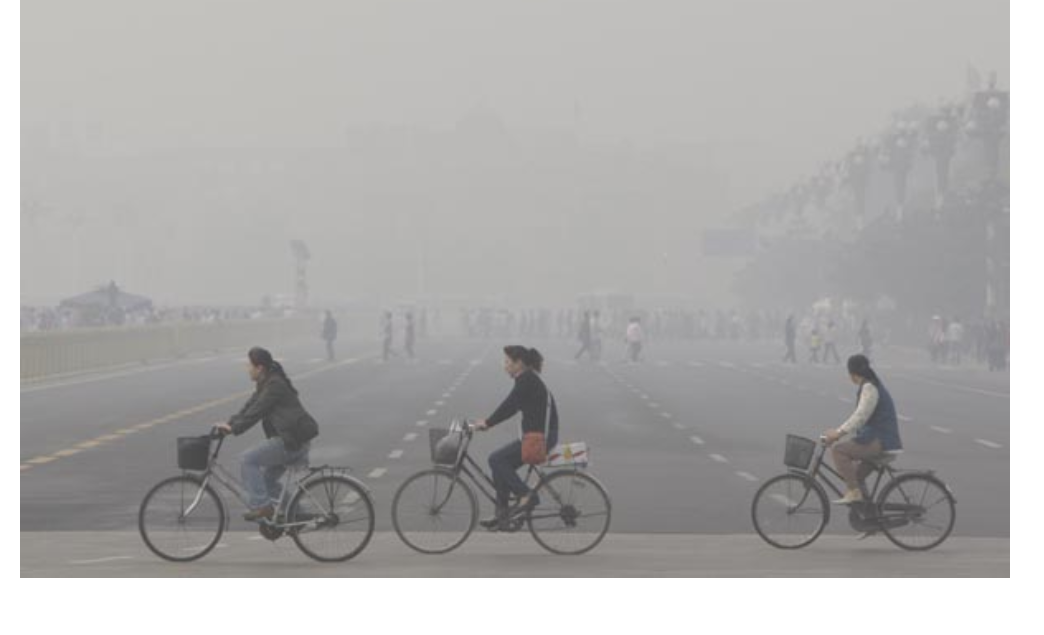
\includegraphics[width=0.82\linewidth]{img/di_fog.png}\end{center}
\ptesub{范文 Model Answer}
\begin{modelbox}
The following graph gives information about the view of a street in fog. This is a very dull picture taken in a fog, for a view of a street. According to this graph, at the central area, there are three bicycles ridden by women at the front and the color of them is black. You can see from this graph that, behind the bicycles, a white, thick blanket of fog covers a lot of people and street lights. What's more, in the background, four straight dashed lines lie on the road, and the color is white. Finally the weather is foggy and the sky is grey.
\end{modelbox}
\zh{下图给出的是大雾中一条街道的景象信息。这是一张在大雾中拍摄、画面非常昏暗的街景照片。根据该图，在中间区域有三辆自行车，骑车的都是女性且在最前面，车的颜色为黑色。从图中可以看到，在自行车后方，一层白色的浓雾笼罩着许多行人和路灯。此外，在背景中，路面上有四条笔直的白色虚线。最后，天气雾蒙蒙，天空呈灰色。}
\ptesub{你的作答（AI 语音识别逐词配色）}
\asrlegend
\begin{asrbox}
\sg{we} \sg{can} \sg{see} \sy{this} \sg{pictures} \sg{shows} \sg{sri} \sg{peoples} \sg{are} \sg{riding} \sg{their} \sg{bikes} \sg{and} \sg{some} \sg{people} \sg{are} \sg{working} \sg{and} \sr{in} \sy{this} \sg{ultimate} \sy{modified} \sy{atmosphere} \sg{is} \sg{not} \sg{good} \sg{and} \sg{we} \sg{cannot} \sg{see} \sg{many} \sy{things} \sg{in} \sg{this} \sg{picture}
\end{asrbox}
\smallskip
{\small\textbf{评分：}内容 \szero{0.6/5} \quad\textperiodcentered\quad 发音 \szero{10/90} \quad\textperiodcentered\quad 流利度 \szero{10/90}}\quad{\footnotesize\color{gray}（录音 0:34，用时 01:00）}
\end{qblock}

% ---------------- Q20 ----------------
\begin{qblock}{Q20\quad DI \#22\ \ Hospital Visits}{描述图 · 总分 \textcolor{cAccent}{\bfseries 25}/90}
\ptesub{配图 Image}
\begin{center}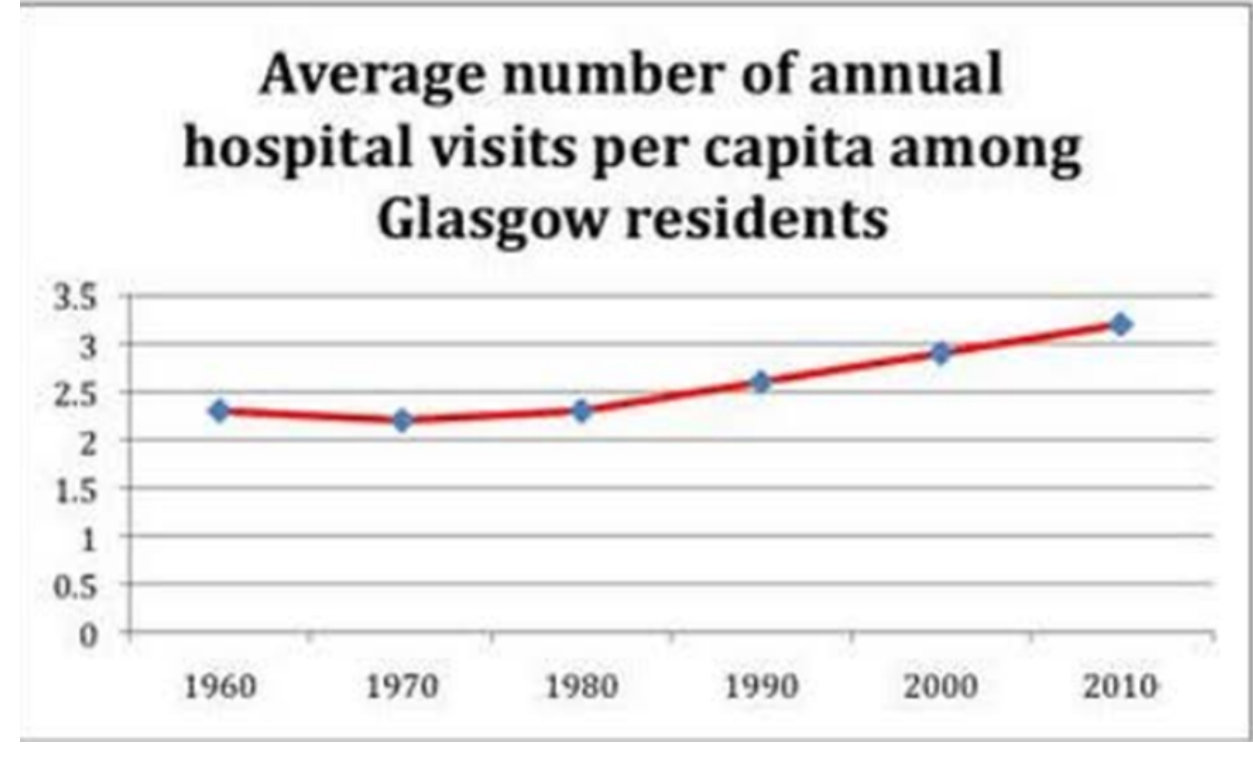
\includegraphics[width=0.85\linewidth]{img/di_hospital.png}\end{center}
\ptesub{范文 Model Answer}
\begin{modelbox}
The following graph gives information about the average number of annual hospital visits per capita among Glasgow residents. The horizontal axis is years, ranging from 1960 to 2010. According to this graph, in 1960, the value is around 2.5. And in 1970, the number is around 2. The highest one is around 3, which is in 2010. On the contrary, the lowest point is around 2, which is in 1970. In conclusion, if this trend continues, the average number of annual hospital visits will keep increasing in the future.
\end{modelbox}
\zh{下图给出的是格拉斯哥居民人均年度就医次数的信息。横轴是年份，从 1960 年到 2010 年。根据该图，1960 年数值约为 2.5；1970 年约为 2。最高点约为 3，出现在 2010 年；相反，最低点约为 2，出现在 1970 年。总之，如果这一趋势持续下去，未来人均年度就医次数将持续增加。}
\ptesub{你的作答（AI 语音识别逐词配色）}
\asrlegend
\begin{asrbox}
\sg{we} \sg{can} \sg{see} \sy{the} \sg{picture} \sg{shows} \sy{average} \sg{number} \sg{of} \sg{annual} \sg{hospital} \sg{visitors} \sg{per} \sg{capital} \sg{among} \sg{last} \sg{road} \sy{residents} \sg{and} \sg{the} \sg{people} \sg{about} \sy{this} \sg{is} \sy{a} \sg{become} \sg{more} \sg{and} \sg{more} \sg{and} \sg{until} \sg{twenty} \sg{one} \sg{twenty} \sg{ten} \sg{it} \sg{has} \sg{been} \sg{so} \sy{thirty} \sg{percent} \sg{of} \sg{it}
\end{asrbox}
\smallskip
{\small\textbf{评分：}内容 \spart{2/5} \quad\textperiodcentered\quad 发音 \spart{33/90} \quad\textperiodcentered\quad 流利度 \spart{20/90}}\quad{\footnotesize\color{gray}（录音 0:29，用时 00:55）}
\end{qblock}

% ---------------- Q21 ----------------
\begin{qblock}{Q21\quad DI \#74\ \ Majors' Number}{描述图 · 总分 \textcolor{cAccent}{\bfseries 65}/90}
\ptesub{配图 Image}
\begin{center}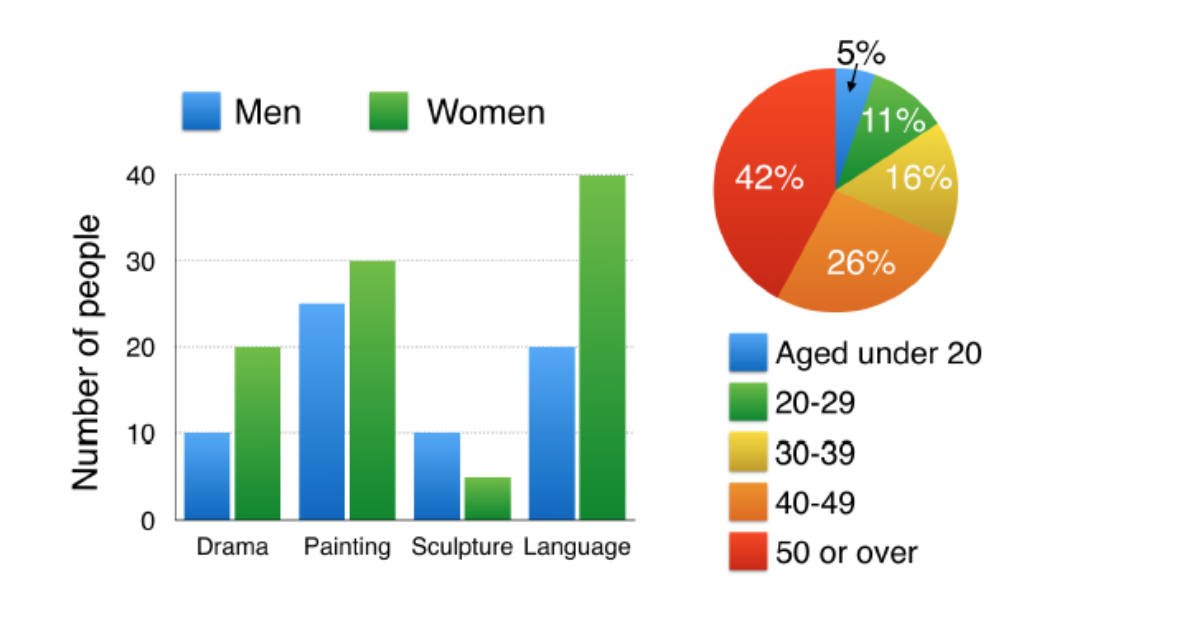
\includegraphics[width=0.97\linewidth]{img/di_majors.png}\end{center}
\ptesub{范文 Model Answer}
\begin{modelbox}
The following graph gives information about the major number. According to this graph, the highest number of people in the language is in women, around 40. On the contrary, the lowest number in painting is in men, which is around 20. And the largest proportion of the age composition is in age over 50, around 42\%. Finally, the smallest percentage is in age under 20, just 5. To sum up, this graph tells about men and women of different ages.
\end{modelbox}
\zh{下图给出的是各专业人数的信息。根据该图，语言专业人数最多的是女性，约为 40 人；相反，绘画专业人数最少的是男性，约为 20 人。年龄构成中占比最大的是 50 岁以上，约 42\%；占比最小的是 20 岁以下，仅 5\%。总而言之，该图讲述了不同年龄段男性和女性的情况。}
\ptesub{你的作答（AI 语音识别逐词配色）}
\asrlegend
\begin{asrbox}
\sg{we} \sg{can} \sg{see} \sy{the} \sg{chart} \sg{shows} \sg{number} \sg{of} \sg{people} \sg{in} \sy{drama} \sg{painting} \sg{sculpture} \sg{and} \sg{the} \sg{language} \sg{we} \sg{can} \sg{see} \sg{drama} \sg{and} \sg{painting} \sy{a} \sy{woman} \sg{become} \sg{more} \sg{and} \sy{the} \sg{sculpture} \sy{a} \sg{man} \sg{get} \sg{more} \sg{and} \sg{we} \sg{can} \sy{see} \sy{the} \sy{left} \sg{child} \sg{is} \sg{a} \sg{h} \sg{under} \sg{twenty} \sg{twenty} \sg{to} \sg{twenty} \sy{nine} \sg{or} \sy{the} \sg{fifty} \sg{or} \sg{over} \sg{and} \sg{fifty} \sg{or} \sg{over} \sy{cost} \sg{the} \sg{most}
\end{asrbox}
\smallskip
{\small\textbf{评分：}内容 \sfull{4.6/5} \quad\textperiodcentered\quad 发音 \sfull{78/90} \quad\textperiodcentered\quad 流利度 \spart{49/90}}\quad{\footnotesize\color{gray}（录音 0:36，用时 01:02）}
\end{qblock}


\ptetask{情景应答}{Respond to a Situation · RTS　Q22--24（评分含恰当性）}
% ---------------- Q22 ----------------
\begin{qblock}{Q22\quad RTS (C) \#26\ \ Checking Presentation Slides}{情景应答 · 总分 \textcolor{cAccent}{\bfseries 38}/90}
\ptesub{情景 Situation}
\begin{promptbox}
Your colleague asks if you can review the presentation slides they've prepared for an upcoming meeting. However, you realize you have several urgent tasks to complete by the end of the day. You need to politely ask for more time to ensure you can give their slides the attention they deserve. What would you say to your colleague?
\end{promptbox}
\zh{你的同事问你能否帮忙看一下他为即将到来的会议准备的演示幻灯片。然而你意识到自己当天还有几项紧急任务要在下班前完成。你需要礼貌地请求多给你一些时间，以确保能认真对待他的幻灯片。你会对同事说什么？}
\ptesub{参考答案 Model Answer}
\begin{modelbox}
Hey, I appreciate you reaching out about the presentation slides. But I have a few urgent tasks to attend to today, so I may not be able to review them thoroughly right away. Would it be possible to have until tomorrow morning to give them a proper look? I want to ensure I can provide valuable feedback. Thanks for understanding!
\end{modelbox}
\zh{嘿，谢谢你来找我看演示幻灯片。不过我今天还有几项紧急任务要处理，所以可能没法马上仔细看。能不能给我到明天早上的时间，让我好好看一看？我想确保能给出有价值的反馈。谢谢你的理解！}
\ptesub{你的作答（AI 语音识别逐词配色）}
\asrlegend
\begin{asrbox}
\sy{hi} \sg{i} \sg{know} \sg{you} \sg{want} \sg{to} \sg{ask} \sg{me} \sg{if} \sg{i} \sg{can} \sg{review} \sg{the} \sg{presentation} \sg{slide} \sg{you} \sg{have} \sy{prepared} \sg{for} \sg{an} \sy{oncoming} \sg{meeting} \sg{but} \sg{however} \sg{i} \sg{realize} \sg{i} \sg{have} \sg{several} \sr{arjun} \sg{test} \sg{to} \sg{complete} \sg{by} \sy{the} \sg{end} \sg{of} \sg{day} \sg{so} \sg{i} \sg{need} \sy{to} \sg{politely} \sg{ask} \sg{for} \sg{more} \sg{time} \sg{to} \sg{ensure} \sg{i} \sg{can} \sg{give} \sg{your} \sg{slide} \sg{and} \sy{attend} \sg{your} \sg{deserve} \sg{so} \sg{please} \sg{give} \sg{me} \sg{the} \sg{time}
\end{asrbox}
\smallskip
{\small\textbf{评分：}恰当性 \spart{53/90} \quad\textperiodcentered\quad 发音 \spart{28/90} \quad\textperiodcentered\quad 流利度 \spart{39/90}}\quad{\footnotesize\color{gray}（录音 0:40，用时 01:30）}
\end{qblock}

% ---------------- Q23 ----------------
\begin{qblock}{Q23\quad RTS (C) \#27\ \ Feasible Options}{情景应答 · 总分 \textcolor{cAccent}{\bfseries 44}/90}
\ptesub{情景 Situation}
\begin{promptbox}
You're planning a weekend getaway with friends, and they're discussing the activities they want to do. However, you realize some of the suggestions might not be feasible due to time constraints or budget limitations. You need to gently guide the conversation towards more realistic options without dampening the excitement. What would you say to your friends?
\end{promptbox}
\zh{你正和朋友们计划一次周末短途出游，他们在讨论想做的各种活动。然而你意识到，由于时间或预算限制，有些建议可能不太可行。你需要在不打击大家热情的前提下，温和地把话题引向更现实的选择。你会对朋友们说什么？}
\ptesub{参考答案 Model Answer}
\begin{modelbox}
Hey everyone, I'm loving all the ideas for our weekend getaway! Just a heads up, I think some of the activities might be a bit tricky to fit into our schedule or budget. How about we brainstorm some alternative options that are more practical but still super fun? We want to make the most of our time together without stressing about logistics. Let's keep the excitement going and find the perfect balance of adventure and affordability!
\end{modelbox}
\zh{嘿，各位，我很喜欢大家为周末出游想到的所有点子！不过提醒一下，我觉得有些活动可能不太好安排进我们的日程或预算。不如我们一起头脑风暴一些更实际但同样超有趣的备选方案？我们想充分利用在一起的时间，而不必为各种安排操心。让我们保持这份兴奋，找到冒险与实惠之间的完美平衡吧！}
\ptesub{你的作答（AI 语音识别逐词配色）}
\asrlegend
\begin{asrbox}
\sy{hi} \sg{i} \sg{notice} \sy{that} \sg{you} \sg{are} \sg{discussing} \sy{the} \sg{activity} \sy{you} \sg{want} \sg{to} \sg{do} \sg{however} \sg{i} \sy{realize} \sg{some} \sg{of} \sg{suggestions} \sg{might} \sr{not} \sg{be} \sg{feasible} \sg{to} \sg{choose} \sg{time} \sg{contrast} \sg{or} \sg{budget} \sg{limitation} \sg{so} \sg{i} \sg{think} \sg{i} \sg{need} \sg{to} \sg{gently} \sy{guides} \sg{the} \sg{conversation} \sr{holds} \sg{more} \sg{relaxed} \sr{iq} \sg{options} \sg{without} \sr{damaging} \sg{the} \sg{excitement} \sg{um} \sg{let's} \sg{let's} \sg{have} \sg{a} \sg{talk}
\end{asrbox}
\smallskip
{\small\textbf{评分：}恰当性 \spart{59/90} \quad\textperiodcentered\quad 发音 \spart{40/90} \quad\textperiodcentered\quad 流利度 \spart{40/90}}\quad{\footnotesize\color{gray}（录音 0:40，用时 01:32）}
\end{qblock}

% ---------------- Q24 ----------------
\begin{qblock}{Q24\quad RTS (C) \#28\ \ Food Choice}{情景应答 · 总分 \textcolor{cAccent}{\bfseries 54}/90}
\ptesub{情景 Situation}
\begin{promptbox}
You're hosting a dinner party for friends, and they're suggesting elaborate dishes that require a lot of preparation. However, you realize you have limited time and resources to cook such elaborate meals. You need to gently steer the conversation towards simpler, yet equally delicious. What would you say to your friends?
\end{promptbox}
\zh{你正在为朋友们举办一场晚餐聚会，他们建议做一些需要大量准备工作的精致菜肴。然而你意识到自己时间和资源有限，没法做这么复杂的大餐。你需要温和地把话题引向更简单却同样美味的选择。你会对朋友们说什么？}
\ptesub{参考答案 Model Answer}
\begin{modelbox}
Hey everyone, I'm excited about our dinner party! Some of the dishes suggested sound amazing, but I'm worried they might be too time-consuming given my schedule. How about we focus on simpler recipes that still pack a punch in flavor? Maybe we can opt for some crowd-pleasers like pasta dishes, grilled meats, or hearty salads that are easy to prepare but still delicious. Let's keep it stress-free and enjoyable for everyone!
\end{modelbox}
\zh{嘿，各位，我对我们的晚餐聚会很期待！有些建议的菜听起来棒极了，但我担心考虑到我的时间安排，它们可能太费工夫了。不如我们专注于一些更简单、但味道依然十足的食谱？也许可以选一些大众喜爱的菜，比如意面、烤肉或丰盛的沙拉，它们做起来简单又好吃。让我们把它办得轻松又愉快吧！}
\ptesub{你的作答（AI 语音识别逐词配色）}
\asrlegend
\begin{asrbox}
\sy{hi} \sg{i} \sg{notice} \sy{that} \sg{you're} \sg{suggestion} \sy{elaborate} \sg{dishes} \sy{that} \sg{require} \sg{a} \sg{lot} \sg{of} \sy{proper} \sg{preparation} \sg{however} \sg{i} \sg{realize} \sg{we} \sg{have} \sy{limited} \sg{time} \sg{and} \sg{resources} \sg{to} \sg{cook} \sg{such} \sy{elaborate} \sg{meals} \sg{so} \sg{i} \sg{think} \sg{we} \sg{should} \sr{think} \sy{a} \sg{generally} \sr{steer} \sg{the} \sg{conversation} \sy{towards} \sg{simpler} \sg{yes} \sy{the} \sr{equal} \sg{delicious} \sg{so} \sg{let's} \sg{have} \sg{a} \sg{talk}
\end{asrbox}
\smallskip
{\small\textbf{评分：}恰当性 \sfull{69/90} \quad\textperiodcentered\quad 发音 \spart{52/90} \quad\textperiodcentered\quad 流利度 \spart{48/90}}\quad{\footnotesize\color{gray}（录音 0:40，用时 01:31）}
\end{qblock}


\ptetask{简短回答}{Answer Short Question · ASQ　Q25--30（单题 0/1）}
\begin{notebox}
{\footnotesize\color{gray}ASQ 考查“听问答词”，单题 0/1。你的录音不收；下表为题目、中文翻译与参考答案（绿）。}
\smallskip\par
\textbf{Q25\quad ASQ \#1358}\quad{\footnotesize\color{gray}（用时 00:19，得分 \sfull{1/1}）}\\
Which is the biggest one, the elephant, the tiger, or the cheetah?\\
\zh{大象、老虎和猎豹，哪一个最大？}\\
参考答案：{\color{cFix}\textbf{Elephant}}（大象）
\par\smallskip
\textbf{Q26\quad ASQ \#1335}\quad{\footnotesize\color{gray}（用时 00:17，得分 \szero{0/1}）}\\
How do we call a person who is about the same age?\\
\zh{我们怎么称呼一个年龄相仿的人？}\\
参考答案：{\color{cFix}\textbf{Contemporary / peer}}（同龄人 / 同辈人）
\par\smallskip
\textbf{Q27\quad ASQ \#1359}\quad{\footnotesize\color{gray}（用时 00:16，得分 \szero{0/1}）}\\
What is the top surface inside the room?\\
\zh{房间内部最上面的那个面叫什么？}\\
参考答案：{\color{cFix}\textbf{Ceiling}}（天花板）
\par\smallskip
\textbf{Q28\quad ASQ \#1376}\quad{\footnotesize\color{gray}（用时 00:17，得分 \szero{0/1}）}\\
What do we call a person who studies mystery?\\
\zh{我们怎么称呼研究神秘事物的人？}\\
参考答案：{\color{cFix}\textbf{Mystic / occult}}（神秘主义者 / 玄学）
\par\smallskip
\textbf{Q29\quad ASQ \#1375}\quad{\footnotesize\color{gray}（用时 00:20，得分 \szero{0/1}）}\\
What do we call the event in which people move through a public place to celebrate an important day or event?\\
\zh{我们把人们穿过公共场所以庆祝重要日子或事件的活动叫什么？}\\
参考答案：{\color{cFix}\textbf{Parade}}（游行）
\par\smallskip
\textbf{Q30\quad ASQ \#1377}\quad{\footnotesize\color{gray}（用时 00:15，得分 \szero{0/1}）}\\
What do we call a diagram in which an object would appear to viewers if it were cut from top to bottom?\\
\zh{把物体从上到下剖开后呈现给观者的图叫什么？}\\
参考答案：{\color{cFix}\textbf{Section}}（剖面图 / 截面）
\end{notebox}

\clearpage
% ===== sec_reading_body.tex =====
% ===================== 阅读 Reading =====================
\ptesection{阅读}{Reading · FIB + MCM-R + RO + FIBD\&D + MCS-R}{46}

\vspace{1mm}
{\small\color{gray} 本部分共 \textbf{16 题}：\textbf{FIB 读写填空}（下拉选词）Q1--5、\textbf{MCM-R 多选}Q6--7、\textbf{RO 段落重排}Q8--9、\textbf{FIBD\&D 读填空}（拖词入空）Q10--14、\textbf{MCS-R 单选}Q15--16。
每题保留文章原文、你的作答（空处对错与平台一致：\rok{绿勾}=选对，{\color{cWrong}\ding{55}}\,红叉=选错并给正确答案）、选项/词库（正确项加粗）、平台中文\textbf{解析}、你的答案与得分；并为每篇文章附\textbf{中文翻译}。本套阅读总分 \textbf{46 / 90}。}
\vspace{2mm}

\newcolumntype{Z}{>{\RaggedRight\arraybackslash}X}

% ---------------- Q1 ----------------
\begin{qblock}{Q1\quad FIB \#386\ \ Product Selling}{读写填空 · 评分 \textcolor{cAccent}{\bfseries 4 / 5}}
\ptesub{文章 Passage（含填空作答）}
\begin{promptbox}
Once an organization has its product to sell, it must then determine the appropriate price to sell it at. The price is set by \rok{balancing} many factors including supply-and-demand, cost, desired profit competition, perceived value, and market behavior. Ultimately, the final price is \rok{determined} by what the market is willing to \rok{exchange} for the product. Pricing theory can be quite complex because so many factors influence what the purchaser decides is a fair \rok{value}.

It also should be \rno{pointed}{noted} that, in addition to monetary exchange, price can be the exchange of goods or services as in a barter agreement, or an exchange of specific behavior, such as a vote in a political campaign.
\end{promptbox}
\zh{一旦组织有了要销售的产品，就必须确定合适的售价。价格由平衡供求、成本、预期利润与竞争、感知价值和市场行为等诸多因素来设定。最终，产品的价格取决于市场愿意为它交换什么。定价理论可能相当复杂，因为有太多因素影响购买者所认为的公平价值。还应注意的是，除了货币交换，价格也可以是货物或服务的交换（如以物易物），或是特定行为的交换，比如在政治竞选中投票。}
\ptesub{选项 Choices（每空 4 选 1，正确项加粗）}
{\small
1.\ comparing,\ begetting,\ \textbf{balancing},\ offsetting\\
2.\ collected,\ mitigated,\ \textbf{determined},\ exhausted\\
3.\ consign,\ design,\ \textbf{exchange},\ prepare\\
4.\ addition,\ shape,\ content,\ \textbf{value}\\
5.\ pointed,\ enlarged,\ overrated,\ \textbf{noted}}
\ptesub{解析 Explanation}
\begin{notebox}\footnotesize
\textbf{1.\ balancing}\quad【思路】The price is set by \_\_\_ many factors including...本句大意：产品价格由"包括……在内的诸多因素"所决定（set by）。首先排除 begetting"引起、导致"和 offsetting"弥补、抵消"，均不搭配宾语"因素"；再看 comparing"对比"和 balancing"平衡"，结合常识，商品价格是多种因素共同作用、综合考虑后做出的，而非对比多种因素，故排除 comparing，选 balancing"平衡多种因素"。【考点】单句理解+单词辨析\par\smallskip
\textbf{2.\ determined}\quad【思路】...the final price is \_\_\_ by what the market is willing to ... for the product. 排除 collected"收集"、mitigated"减轻"、exhausted"耗尽"（代入说不通），只有 determined"决定"与 price 搭配。【考点】单句理解+单词辨析\par\smallskip
\textbf{3.\ exchange}\quad【思路】...what the market is willing to \_\_\_ for the product. 市场愿意用什么东西换该产品；consign"寄存/委托"、design"设计"、prepare"准备"均不合，市场交易即以物换物或以钱换物，故选 exchange。【考点】单句理解+词意辨析\par\smallskip
\textbf{4.\ value}\quad【思路】...what the purchaser decides is a fair \_\_\_ . 句中已出现"因素"，空格应填表"定价"的名词；addition"增添物"、shape"形状"、content"内容"均不合，选 value"价值、价格"。【考点】上下文理解+单词辨析\par\smallskip
\textbf{5.\ noted}\quad【思路】It also should be \_\_\_ that, ... 选项中 pointed"被指"无引导 that 从句的用法；enlarged"增大"、overrated"高估"均说不通；只有 noted"注意"合适。【考点】单句理解+单词辨析
\end{notebox}
\smallskip
\textbf{你的答案：}\ balancing, determined, exchange, value, {\color{cWrong}pointed}\qquad\textbf{本题得分：}\ {\color{cAccent}\bfseries 4 / 5}\quad{\footnotesize\color{gray}（用时 02:50；第 5 空 pointed→noted）}
\end{qblock}

% ---------------- Q2 ----------------
\begin{qblock}{Q2\quad FIB \#387\ \ Green Spaces}{读写填空 · 评分 \textcolor{cAccent}{\bfseries 3 / 4}}
\ptesub{文章 Passage（含填空作答）}
\begin{promptbox}
Green spaces contribute significantly to a \rok{reduction} in soil and aerial temperatures during spells of hot weather, so contributing to human wellbeing. In the garden \rok{context}, there is, however, little information as to what extent various types of plants \rno{defer}{differ} in their cooling potential and how certain planting combinations may maximize cooling under a scenario of \rok{low} rainfall and minimal water inputs.
\end{promptbox}
\zh{在炎热天气期间，绿地能显著降低土壤和空气的温度，从而有益于人类福祉。然而，在园林环境中，关于不同类型的植物在冷却潜力方面有多大差异、以及在低降雨量和最少水输入的情景下哪些植物组合能最大化降温，相关信息却很少。}
\ptesub{选项 Choices（每空 4 选 1，正确项加粗）}
{\small
1.\ genesis,\ conclusion,\ purification,\ \textbf{reduction}\\
2.\ background,\ level,\ \textbf{context},\ volume\\
3.\ confer,\ \textbf{differ},\ alternate,\ defer\\
4.\ total,\ \textbf{low},\ parallel,\ dropped}
\ptesub{解析 Explanation}
\begin{notebox}\footnotesize
\textbf{1.\ reduction}\quad【思路】绿地有利于\_\_\_土壤和空气的温度，据后文 so contributing to human wellbeing，炎热天气下降温对人更好，故在 genesis(起源)/conclusion(总结)/purification(净化)/reduction(减少) 中只能选 reduction。【考点】上下文理解\par\smallskip
\textbf{2.\ context}\quad【思路】In the garden \_\_\_, there is...；background"背景"、level"水平"、volume"体积/音量"均说不通，只有 context"环境"合适，in the garden context 即"在花园环境中"。【考点】词义辨析\par\smallskip
\textbf{3.\ differ}\quad【思路】as 做连词连接前后两句，主语 various types of plants，空格为谓语动词；常识可判断"不同植物的冷却潜力是不同的"，故在 confer(商讨/授予)/differ(不同于)/alternate(交替)/defer(推迟) 中只有 differ 能表达"不同"。【考点】句意理解\par\smallskip
\textbf{4.\ low}\quad【思路】under a scenario of \_\_\_ rainfall and minimal water inputs；and 连接两个名词词组，空格要与 minimal 对应表"少的、低的"，在 total/low/parallel/dropped 中选 low，搭配 rainfall 即"最少的降雨量"。【考点】并列结构
\end{notebox}
\smallskip
\textbf{你的答案：}\ reduction, context, {\color{cWrong}defer}, low\qquad\textbf{本题得分：}\ {\color{cAccent}\bfseries 3 / 4}\quad{\footnotesize\color{gray}（用时 02:17；第 3 空 defer→differ）}
\end{qblock}

% ---------------- Q3 ----------------
\begin{qblock}{Q3\quad FIB \#28\ \ Guide Stick}{读写填空 · 评分 \textcolor{cAccent}{\bfseries 3 / 5}}
\ptesub{文章 Passage（含填空作答）}
\begin{promptbox}
Foldable white canes help the \rno{insensitivity}{visually} impaired navigate their surroundings. But the guide stick's tactile nature offers only so much information. The cane's user must manually find and avoid obstructions. But new high-tech canes are on the horizon.

Last year researchers in India tried to fill in some of the missing info with their experimental SmartCane. The device uses an attached ultrasonic transmitter and a sensor that vibrates the cane to warn its users when an obstacle is within three meters.

Students at the U.K.'s Birmingham City University are developing a cane that can even identify acquaintances as they \rok{approach}. Called the `XploR' mobility cane, it includes an \rno{skinhead}{embedded} digital camera that analyzes the faces of people walking by and compares their images against a database stored on a memory card in the cane's handle.

If there's a facial recognition match, the cane alerts the user's \rok{smartphone} via Bluetooth. The phone then identifies the approaching person to the user via its speaker or earbuds. The \rok{students} are building a prototype they'll test later this year.

The hurdles are significant: facial recognition is a tough problem, especially outdoors. But if the XploR works, it could actually give the visually impaired a leg up on everyone else --- especially those of us who never remember people's names.
\end{promptbox}
\zh{可折叠的白手杖帮助视障者在周围环境中导航，但手杖触觉所能提供的信息有限，使用者必须手动寻找并避开障碍物——不过新型高科技手杖即将问世。去年印度研究人员用实验性的 SmartCane 试图补上一些缺失信息：该设备装有超声波发射器和传感器，当障碍物进入三米内时震动手杖以警示用户。英国伯明翰城市大学的学生正在研发一种甚至能在熟人走近时辨认出他们的手杖。这款名为"XploR"的移动手杖内置嵌入式数码相机，分析路过者面部，并与手杖手柄记忆卡中的数据库比对。一旦匹配成功，手杖通过蓝牙提醒用户的智能手机，手机再经扬声器或耳机告知走近的人是谁。这些学生正在制作原型，将于今年晚些时候测试。难点不小：面部识别是个难题，尤其在户外；但若 XploR 成功，它真能让视障者比常人更有优势——尤其对我们这些总记不住名字的人。}
\ptesub{选项 Choices（每空 4 选 1，正确项加粗）}
{\small
1.\ felicity,\ insensitivity,\ \textbf{visually},\ malleability\\
2.\ likelihood,\ throat,\ northernmost,\ \textbf{approach}\\
3.\ untested,\ \textbf{embedded},\ deadest,\ skinhead\\
4.\ waterborne,\ alone,\ \textbf{smartphone},\ postpone\\
5.\ jurisprudence,\ bootless,\ \textbf{students},\ jukebox}
\ptesub{解析 Explanation}
\begin{notebox}\footnotesize
\textbf{1.\ visually}\quad【思路】help the \_\_\_ impaired navigate...；考察 the+形容词表名词（如 the rich），the impaired 指健康受损者，故选副词 visually，the visually impaired 即"视障者"。felicity n.幸福、insensitiveness n.不灵敏、malleability n.可锻性，词性词义均不符。【考点】副词；单句理解\par\smallskip
\textbf{2.\ approach}\quad【思路】...identify acquaintances as they \_\_\_，as 从句缺谓语，选动词；throat"用喉音"不合，approach"接近"，表达熟人走近时可辨认。【考点】从句；单句理解\par\smallskip
\textbf{3.\ embedded}\quad【思路】includes an \_\_\_ digital camera...；an 说明元音开头，untested"未经检验的"与后文"已用于分析比较"矛盾排除，手杖小巧、相机需嵌入才实用，选 embedded"嵌入的"。【考点】形容词+名词结构；单句理解\par\smallskip
\textbf{4.\ smartphone}\quad【思路】alerts the user's \_\_\_ via Bluetooth；受 user's 修饰、缺宾语，应选名词且为用户所有物，waterborne/alone/postpone 均不合，选 smartphone。【考点】单句理解\par\smallskip
\textbf{5.\ students}\quad【思路】The \_\_\_ are building a prototype...；系动词 are 前缺复数主语，只有 students"学生"符合；jurisprudence 法律学、bootless 无用的、jukebox 自动点唱机均不符。【考点】主谓一致；单句理解
\end{notebox}
\smallskip
\textbf{你的答案：}\ {\color{cWrong}insensitivity}, approach, {\color{cWrong}skinhead}, smartphone, students\qquad\textbf{本题得分：}\ {\color{cAccent}\bfseries 3 / 5}\quad{\footnotesize\color{gray}（用时 03:21；第 1 空 insensitivity→visually、第 3 空 skinhead→embedded）}
\end{qblock}

% ---------------- Q4 ----------------
\begin{qblock}{Q4\quad FIB \#33\ \ Clown Fish}{读写填空 · 评分 \textcolor{cAccent}{\bfseries 3 / 5}}
\ptesub{文章 Passage（含填空作答）}
\begin{promptbox}
Clown fish became famous thanks to the movie Finding Nemo. In real life, their social hierarchy is simple: larger fish dominate their smaller \rno{palms}{counterparts}. Now we know that to reinforce this social structure, the fish communicate with aggressive and submissive audio signals. The new info is in the journal PLoS ONE.

Researchers \rok{recorded} clown fish calls, \rok{capturing} this noise as one chased a smaller fish. These popping sounds function as an aggression signal. When a clown fish has been chased and wishes to submit, it shakes its head in a submissive gesture and produces clicking noises like these. The researchers \rok{compared} the aggressive and submissive calls, and found that the sound pulses in a submissive signal were shorter and more high-pitched.

Unlike many animals that use sound to draw in \rno{exponential}{potential} mates, clown fish appear to use their calls only as labels of social status. When a little fish makes submissive sounds to a larger one, neither has to invest in a physical confrontation. Which is good news for small-fry like Nemo.
\end{promptbox}
\zh{小丑鱼因电影《海底总动员》而出名。现实中它们的社会等级很简单：大鱼支配小鱼。如今我们知道，为强化这种结构，小丑鱼通过攻击性与顺从性的声音信号沟通（新发现见期刊 PLoS ONE）。研究人员录下了小丑鱼的叫声，捕捉到一条鱼追逐另一条小鱼时的声音；这些"砰砰"声起攻击信号的作用。当一条小丑鱼被追逐并想示弱时，它会摆头做顺从姿态并发出类似咔嗒声。研究人员比较了攻击性与顺从性叫声，发现顺从信号的声脉冲更短、音调更高。与许多用声音吸引潜在配偶的动物不同，小丑鱼似乎只把叫声当作社会地位的标签。当小鱼向大鱼示弱发声时，双方都无需肢体冲突——这对像尼莫这样的小鱼是个好消息。}
\ptesub{选项 Choices（每空 4 选 1，正确项加粗）}
{\small
1.\ palms,\ prompts,\ traps,\ \textbf{counterparts}\\
2.\ unfolded,\ deported,\ \textbf{recorded},\ dialed\\
3.\ cluttering,\ profiting,\ \textbf{capturing},\ padlocking\\
4.\ pared,\ \textbf{compared},\ guided,\ treaded\\
5.\ exponential,\ \textbf{potential},\ nimble,\ ventral}
\ptesub{解析 Explanation}
\begin{notebox}\footnotesize
\textbf{1.\ counterparts}\quad【思路】冒号后是对前面 social hierarchy 的具体说明（大鱼统治小鱼），与 larger fish 相对应的是小鱼，故选 counterparts"对应的事物"；palms"手掌/棕榈"、prompts"提示符"、traps"陷阱"均不恰当。【考点】词义辨析；单句理解\par\smallskip
\textbf{2.\ recorded}\quad【思路】Researchers \_\_\_ clown fish calls...；unfold"揭露"、deport"驱逐"、dial"拨号"按宾语 clown fish calls 排除，record"记录/录制"最合。【考点】动宾搭配\par\smallskip
\textbf{3.\ capturing}\quad【思路】逗号前已是完整主谓宾，考察现在分词作伴随状语；this noise 即 calls，capture"捕捉"与 record calls 可作伴随动作；clutter/profit/padlock 均不合。【考点】现在分词；单句理解\par\smallskip
\textbf{4.\ compared}\quad【思路】空格动词与 and found 并列；后文 were shorter and more high-pitched 有比较级，说明对比了两种叫声，故选 compare；pare"去皮"、guide"引导"、tread"踩踏"不合。【考点】并列关系；动宾搭配\par\smallskip
\textbf{5.\ potential}\quad【思路】修饰名词 mates，draw in 表"吸引"；exponential"成指数的"、nimble"灵活的"、ventral"腹部的"均不合，吸引"潜在的"伴侣最通顺，选 potential。【考点】搭配；单句理解
\end{notebox}
\smallskip
\textbf{你的答案：}\ {\color{cWrong}palms}, recorded, capturing, compared, {\color{cWrong}exponential}\qquad\textbf{本题得分：}\ {\color{cAccent}\bfseries 3 / 5}\quad{\footnotesize\color{gray}（用时 02:19；第 1 空 palms→counterparts、第 5 空 exponential→potential）}
\end{qblock}

% ---------------- Q5 ----------------
\begin{qblock}{Q5\quad FIB \#79\ \ Wind}{读写填空 · 评分 \textcolor{cAccent}{\bfseries 4 / 5}}
\ptesub{文章 Passage（含填空作答）}
\begin{promptbox}
The world's atmosphere is forever on the move. Wind is air in motion. Sometimes air moves slowly, giving a gentle breeze. At other times it moves rapidly, creating gales and hurricanes. \rok{Gentle} or fierce, wind always starts in the same way. As the sun moves through the sky, it heats up some parts of the sea and land more than others. The air above these \rok{hot} spots is warmed, becomes lighter than the surrounding air, and begins to rise. Elsewhere, cool air sinks, because it is \rok{heavier}. Winds blow because air squeezed out by sinking, cold air is sucked in under rising, warm air. Winds will blow wherever there is a \rno{diversity}{difference} in air temperature and pressure, always flowing from high to low pressure. Some winds blow in one place, and have a local name --- North America's chinook and France's mistral. Others are part of a huge circulation pattern that sends winds over the \rok{entire} globe.
\end{promptbox}
\zh{地球大气永远在运动，风就是运动中的空气。有时空气缓慢移动形成微风，有时快速移动形成大风和飓风。无论温和还是猛烈，风总以同样方式开始。太阳划过天空，对海陆某些部分的加热多于他处；这些热点上方的空气被加热、变得比周围空气轻而上升。别处冷空气因更重而下沉。风之所以吹，是因为下沉冷空气被挤出、又被吸入上升暖空气之下。只要空气的温度与气压存在差异，风就会吹，总是从高压流向低压。有些风只在一处吹并有当地名称——如北美的钦诺克风、法国的密史脱拉风；另一些则是把风吹遍全球的巨大环流模式的一部分。}
\ptesub{选项 Choices（每空 4 选 1，正确项加粗）}
{\small
1.\ convergence,\ diversity,\ discretion,\ \textbf{difference}\\
2.\ \textbf{entire},\ all,\ total,\ wholesome\\
3.\ \textbf{heavier},\ deeper,\ larger,\ colder\\
4.\ cold,\ \textbf{hot},\ cool,\ warm\\
5.\ \textbf{Gentle},\ Wild,\ Chill,\ Aloud}
\ptesub{解析 Explanation}
\begin{notebox}\footnotesize
\textbf{1.\ Gentle}\quad【思路】\_\_\_ or fierce, wind always starts...；句首 or 并列的两个形容词意思相反产生对比，只有 gentle"温和的"与 fierce"猛烈的"为反义；Wild/Aloud/Chill 排除。（小技巧：选项中某词与其余三词情感色彩明显不同时，常为正确项。）【考点】前后文联系、词义辨析\par\smallskip
\textbf{2.\ hot}\quad【思路】The air above these \_\_\_ spots is warmed；后文 is warmed 说明气体经热的地方升温，排除 cold/cool；hot 温度更高，其上方温度才会是 warm，故选 hot。【考点】前后文联系、词义辨析\par\smallskip
\textbf{3.\ heavier}\quad【思路】cool air sinks, because it is \_\_\_；明显因果，冷空气下沉只有 heavier"更重"直接满足该逻辑，呼应前文气体变轻上升；deeper/larger/colder 排除。【考点】前后文联系、因果关系\par\smallskip
\textbf{4.\ difference}\quad【思路】wherever there is a \_\_\_ in air temperature and pressure, always flowing from high to low pressure；风从高压往低压走，说明不同压力造成风向不同，选 difference"差异"；convergence/discretion/diversity 不合逻辑。【考点】单句理解\par\smallskip
\textbf{5.\ entire}\quad【思路】sends winds over the \_\_\_ globe；wholesome"健全的"与 globe 搭配不当，total 强调数量总量、all 形容具体事物（all the students），entire"完整的"可修饰抽象名词 globe，故选 entire。【考点】词义辨析、单句理解
\end{notebox}
\smallskip
\textbf{你的答案：}\ Gentle, hot, heavier, {\color{cWrong}diversity}, entire\qquad\textbf{本题得分：}\ {\color{cAccent}\bfseries 4 / 5}\quad{\footnotesize\color{gray}（用时 03:20；第 4 空 diversity→difference）}
\end{qblock}

% ---------------- Q6 ----------------
\begin{qblock}{Q6\quad MCM-R \#117\ \ Ancient DNA}{多选 · 评分 \textcolor{cAccent}{\bfseries 0 / 2}}
\ptesub{文章 Passage}
\begin{promptbox}
Analysis of ancient DNA from one of the best-preserved Neolithic tombs in Britain has revealed that most of the people buried there were from five continuous generations of a single extended family.

By analyzing DNA extracted from the bones and teeth of 35 individuals entombed at Hazleton North long cairn in the Cotswolds-Severn region, the research team was able to detect that 27 of them were close biological relatives. The group lived approximately 5700 years ago -- around 3700-3600 BC -- around 100 years after farming had been introduced to Britain.

Published in Nature, it is the first study to reveal in such detail how prehistoric families were structured, and the international team of archaeologists and geneticists say that the results provide new insights into kinship and burial practices in Neolithic times.
\end{promptbox}
\zh{对英国保存最完好的新石器时代墓葬之一的古 DNA 分析显示，葬于此处的人大多来自同一个大家族连续五代的成员。研究团队分析了科茨沃尔德-塞文地区 Hazleton North 长石冢中 35 个个体的骨骼与牙齿 DNA，发现其中 27 人是近亲。该群体生活在约 5700 年前（约公元前 3700--3600 年），约在农业传入英国 100 年后。该研究发表于《自然》，是首个如此详细揭示史前家庭结构的研究；这支国际团队表示，结果为新石器时代的亲属关系与丧葬习俗提供了新见解。}
\ptesub{题目 Question}
\begin{notebox}What has been revealed by analysis of ancient DNA from one of Britain's best-preserved Neolithic tombs?\end{notebox}
\ptesub{选项 Choices（正确项绿色加粗）}
{\small
A) The results provide new insights into neolithic art.\\
{\color{cFix}\textbf{B) More than half of them were close relatives.}}\\
C) Agriculture hadn't been invented when the group were living.\\
D) All of the people buried in the neolithic tombs are descended from five generations of one extended family.\\
{\color{cFix}\textbf{E) It reveals the details of the organization of the prehistoric family.}}}
\smallskip
\textbf{正确答案}\ \textcolor{cFix}{\bfseries B, E}\qquad\textbf{你的答案}\ {\color{cWrong}\bfseries D}\qquad\textbf{本题得分：}\ {\color{cAccent}\bfseries 0 / 2}\quad{\footnotesize\color{gray}（用时 02:16）}
\end{qblock}

% ---------------- Q7 ----------------
\begin{qblock}{Q7\quad MCM-R \#119\ \ Television}{多选 · 评分 \textcolor{cAccent}{\bfseries 2 / 2}}
\ptesub{文章 Passage}
\begin{promptbox}
There's bad news for parents who frequently plop their kids in front of the TV to give themselves a break: It might actually end up leaving moms and dads more stressed.

Why? Because the more television that kids watch, the more they're exposed to advertising messages. The more advertising they see, the more likely they are to insist on purchasing items when they go with their parents to the store -- and perhaps make a fuss if told ``no.'' All that, researchers say, may contribute to parents' overall stress levels, well beyond a single shopping trip.

The findings come from a University of Arizona-led study, published in the International Journal of Advertising, that explores the potential effects of children's television watching habits on their parents' stress levels.

``The more advertising children see, the more they ask for things and the more conflict is generated,'' said lead study author Matthew Lapierre, an assistant professor in the UArizona Department of Communication in the College of Social and Behavioral Sciences. ``What we haven't looked at before is what the potential effect is on parents. We know kids ask for things, we know it leads to conflict, but we wanted to ask the next question: Could this be contributing to parents' overall stress?'' The study suggests that it could. There are a few things parents can do, perhaps the most obvious of which is limiting screen time.
\end{promptbox}
\zh{对于经常把孩子丢在电视前以求清闲的父母来说，有个坏消息：这样做最终可能让爸妈更焦虑。为什么？因为孩子看的电视越多，接触的广告越多；看的广告越多，就越可能在和父母逛商店时坚持要买东西——被拒绝还可能大吵大闹。研究人员说，这一切都会加重父母的整体压力，远不止一次购物。该发现来自亚利桑那大学主导、发表于《国际广告期刊》的研究，探讨儿童看电视习惯对父母压力的潜在影响。主要作者、传播系助理教授 Matthew Lapierre 说："孩子看的广告越多，要的东西越多，冲突也越多。我们以前没研究过对父母的潜在影响……我们想问：这会不会加重父母的整体压力？"研究表明确实可能。父母能做的事中，最明显的或许是限制屏幕时间。}
\ptesub{题目 Question}
\begin{notebox}What can we infer from the passage?\end{notebox}
\ptesub{选项 Choices（正确项绿色加粗）}
{\small
A) When watching one television ad, children purchase one thing from it.\\
{\color{cFix}\textbf{B) Children will ask for more things when they watch more ads, which can lead to more conflict.}}\\
C) Children's habit of watching TV has definitely no impact on parents' stress level.\\
D) For parents, putting their children in front of the TV tends to make themselves happy.\\
{\color{cFix}\textbf{E) Parents can reduce their stress by limiting their children in watching TV.}}}
\smallskip
\textbf{正确答案}\ \textcolor{cFix}{\bfseries B, E}\qquad\textbf{你的答案}\ \textcolor{cFix}{\bfseries B, E}\qquad\textbf{本题得分：}\ {\color{cAccent}\bfseries 2 / 2}\quad{\footnotesize\color{gray}（用时 02:27，全对）}
\end{qblock}

% ---------------- Q8 ----------------
\begin{qblock}{Q8\quad RO \#361\ \ Research Report}{段落重排 · 评分 \textcolor{cAccent}{\bfseries 2 / 4}}
\ptesub{乱序段落 Paragraphs}
\begin{promptbox}
\textbf{1)} In fact, this final stage -- writing up your research -- may be one of the most difficult.\\
\textbf{2)} I know you won't want to hear this, but your work is still far from done.\\
\textbf{3)} And, in many research projects you will need to write multiple reports that present the results at different levels of detail for different audiences.\\
\textbf{4)} So now that you've completed the research project, what do you do?\\
\textbf{5)} Developing a good, effective and concise report is an art form in itself.
\end{promptbox}
\zh{（按正确顺序）你已完成研究项目，接下来该做什么？——我知道你不爱听，但工作还远未完成；事实上，撰写研究报告这一最后阶段可能是最难的；写出好的、有效且简洁的报告本身就是一门艺术；而且在许多项目里，你还要为不同受众写多份详略不同的报告。}
\smallskip
\textbf{正确顺序}\ \textcolor{cFix}{\bfseries 4 → 2 → 1 → 5 → 3}\qquad\textbf{你的顺序}\ {\color{cWrong}\bfseries 5 → 4 → 2 → 1 → 3}\qquad\textbf{本题得分：}\ {\color{cAccent}\bfseries 2 / 4}\quad{\footnotesize\color{gray}（用时 02:20）}
\end{qblock}

% ---------------- Q9 ----------------
\begin{qblock}{Q9\quad RO \#24\ \ Inuit}{段落重排 · 评分 \textcolor{cAccent}{\bfseries 3 / 3}}
\ptesub{乱序段落 Paragraphs}
\begin{promptbox}
\textbf{1)} Young children don't possess these qualities and are easily angered, cry frequently and are incapable of understanding the external difficulties facing the community, such as shortages of food.\\
\textbf{2)} Jean Briggs has worked with the Inuit of the Canadian Arctic and has described how, within these communities, growing up is largely seen as a process of acquiring thought, reason and understanding (known in Inuit as ihuma).\\
\textbf{3)} It's only when they are older and begin to acquire thought that parents attempt to teach them or discipline them.\\
\textbf{4)} Because they can't be reasoned with, and don't understand, parents treat them with a great deal of tolerance and leniency.
\end{promptbox}
\zh{（按正确顺序）Jean Briggs 与加拿大北极的因纽特人共事，描述了在这些社区里，成长被视为获得思想、理性与理解（因纽特语 ihuma）的过程；幼儿不具备这些品质，易怒、常哭，无法理解社区面临的外部困难（如食物短缺）；因为无法跟他们讲道理、他们也不理解，父母对他们极为宽容忍让；只有当他们长大、开始获得思想时，父母才会尝试教导或管教。}
\smallskip
\textbf{正确顺序}\ \textcolor{cFix}{\bfseries 2 → 1 → 4 → 3}\qquad\textbf{你的顺序}\ \textcolor{cFix}{\bfseries 2 → 1 → 4 → 3}\qquad\textbf{本题得分：}\ {\color{cAccent}\bfseries 3 / 3}\quad{\footnotesize\color{gray}（用时 00:54，全对）}
\end{qblock}

% ---------------- Q10 ----------------
\begin{qblock}{Q10\quad FIBD\&D \#540\ \ Shrimp Farms}{读填空（拖词）· 评分 \textcolor{cAccent}{\bfseries 0 / 4}}
\ptesub{文章 Passage（含填空作答）}
\begin{promptbox}
Over the past two decades around a third of the world's mangrove swamps have been \rno{comprised}{converted} for human use, with many turned into valuable shrimp farms. In 2007 an economic study of such shrimp farms in Thailand showed that the commercial profits per hectare were \$9,632. If that were the only factor, conversion would seem an excellent idea.

However, proper \rno{study}{accounting} shows that for each hectare government subsidies formed \$8,412 of this figure and there were costs, too: \$1,000 for pollution and \$12,392 for losses to ecosystem services. These \rno{productivity}{comprised} damage to the supply of foods and medicines that people had taken from the forest, the loss of habitats for fish, and less buffering against storms. And because a given shrimp farm only stays \rno{accounting}{productive} for three or four years, there was the additional cost of restoring them afterwards.
\end{promptbox}
\zh{过去二十年里，全球约三分之一的红树林沼泽被转作人类用途，许多变成了有利可图的养虾场。2007 年一项对泰国此类养虾场的经济研究显示，每公顷商业利润为 9,632 美元；若这是唯一因素，转化似乎是个绝佳主意。然而恰当核算表明，政府补贴占了其中 8,412 美元，且还有成本：1,000 美元用于污染、12,392 美元用于生态系统服务损失。这些损失包括人们从森林获取的食物和药品供应受损、鱼类栖息地丧失、对风暴的缓冲减弱。又因为一个养虾场只能维持三四年产出，之后还要付出修复的额外成本。}
\ptesub{词库 Word Bank（拖词入空，正确答案加粗）}
{\small 1) regenerating\quad 2) study\quad 3) estimated\quad 4) \textbf{accounting}\quad 5) productivity\quad 6) \textbf{productive}\quad 7) \textbf{converted}\quad 8) \textbf{comprised}}
\ptesub{解析 Explanation}
\begin{notebox}\footnotesize
\textbf{1.\ converted}\quad【思路】...mangrove swamps have been \_\_\_ for human use, with many turned into shrimp farms；前后可推断红树林被人类所用，with 也进一步解释"人们把红树林变成养虾场"；表被动的动词 estimated"估计"、converted"转化"、comprised"组成"中，只有 converted 说得通。【考点】单句理解\par\smallskip
\textbf{2.\ accounting}\quad【思路】However, proper \_\_\_ shows that...；空格在形容词 proper 后、谓语 shows 为三单，应填名词；study 仅在"学习"时不可数，productivity"生产力"代入不通顺，故选 accounting"核算"。【考点】主谓一致+单词辨析\par\smallskip
\textbf{3.\ comprised}\quad【思路】These \_\_\_ damage to the supply of foods and medicines...；these 是主语、damage 是宾语，中间应填动词作谓语；study/estimated/comprised 中只有 comprised"包括"说得通。【考点】单句理解\par\smallskip
\textbf{4.\ productive}\quad【思路】a given shrimp farm only stays \_\_\_ for three or four years；stay 为半系动词，接形容词/副词表"保持……状态"；study/productivity/productive 中，虾场不可能"继续是学习/生产力"，故选 productive，即"虾场仅能在 3--4 年保持产出"。【考点】单句理解
\end{notebox}
\smallskip
\textbf{你的答案：}\ {\color{cWrong}comprised, study, productivity, accounting}\qquad\textbf{本题得分：}\ {\color{cAccent}\bfseries 0 / 4}\quad{\footnotesize\color{gray}（用时 01:58；四空全错，正确为 converted / accounting / comprised / productive）}
\end{qblock}

% ---------------- Q11 ----------------
\begin{qblock}{Q11\quad FIBD\&D \#22\ \ Professional Astronomers}{读填空（拖词）· 评分 \textcolor{cAccent}{\bfseries 1 / 5}}
\ptesub{文章 Passage（含填空作答）}
\begin{promptbox}
Professional astronomers, \rno{equipped}{unlike} their amateur counterparts, have no particular interest in the aesthetic quality of their photographs. What \rno{concerns}{matters} to them is the contribution their images can \rno{use}{make} to research, and to the \rok{collection} of data scientists in their field \rno{make}{use} for research purposes.
\end{promptbox}
\zh{职业天文学家与业余天文学家不同，他们对照片的美学质量并无特别兴趣。对他们来说重要的是，他们的图像能为研究、以及为本领域数据科学家所做的数据采集作出怎样的贡献，并供研究之用。}
\ptesub{词库 Word Bank（拖词入空，正确答案加粗）}
{\small 1) \textbf{make}\quad 2) equipped\quad 3) \textbf{unlike}\quad 4) \textbf{matters}\quad 5) \textbf{use}\quad 6) \textbf{collection}\quad 7) put\quad 8) concerns}
\ptesub{解析 Explanation}
\begin{notebox}\footnotesize
\textbf{1.\ unlike}\quad【思路】Professional astronomers, \_\_\_ their amateur counterparts, ...；该短语前后皆逗号、是主干完整句中的插入语，应选介词，只有 unlike"不像"；amateur 与 professional 相对立也可判断。【考点】介词；单句理解\par\smallskip
\textbf{2.\ matters}\quad【思路】What \_\_\_ to them is the contribution...；what 引导主语从句缺谓语，主句谓语单数 is，故选三单动词；matters/concerns 中，搭配介词 to（matter to sb.）常见，而 concern 为及物动词不搭 to，故选 matters。【考点】主谓一致；单句理解\par\smallskip
\textbf{3.\ make}\quad【思路】the contribution (that) their images can \_\_\_ to research；情态动词 can 后接动词原形；make/use/put 中，与 contribution 搭配只有 make，构成 make contribution to"对……做贡献"。【考点】定语从句；固定搭配；单句理解\par\smallskip
\textbf{4.\ collection}\quad【思路】and to the \_\_\_ of data scientists in their field；名词 of 结构（A of B）应填名词；collection/use/concerns 中，全文主旨是图像对天文学家的作用——能促进数据采集而非使用，故选 collection"采集"。【考点】名词 of 结构；上下文理解\par\smallskip
\textbf{5.\ use}\quad【思路】scientists in their field \_\_\_ for research purposes（省略 that 的从句，修饰 data），缺谓语、主语 scientists 为复数，应填动词原形；use/put 中，作用对象是 data，"使用数据"比"安置数据"恰当，选 use。【考点】定语从句；主谓一致；动宾搭配
\end{notebox}
\smallskip
\textbf{你的答案：}\ {\color{cWrong}equipped, concerns, use}, collection, {\color{cWrong}make}\qquad\textbf{本题得分：}\ {\color{cAccent}\bfseries 1 / 5}\quad{\footnotesize\color{gray}（用时 01:10；仅第 4 空 collection 正确）}
\end{qblock}

% ---------------- Q12 ----------------
\begin{qblock}{Q12\quad FIBD\&D \#31}{读填空（拖词）· 评分 \textcolor{cAccent}{\bfseries 1 / 5}}
{\footnotesize\color{gray} 注：原图本题标题处留空（平台仅重复显示题型 ``FIBD\&D''），下文按内容暂记为 De Quincey / Forgetting。}
\ptesub{文章 Passage（含填空作答）}
\begin{promptbox}
Thomas De Quincey once said that there is no such thing as forgetting --- a rather frightening \rno{information}{thought}. If we could remember everything all the time, not to \rno{say}{mention} those things we feel \rok{ashamed} or guilty about, life would be unbearable. Naturally, we remember shocking and dramatic events better than any \rno{mention}{others}. The things we most often forget are names, numbers, dates, \rno{theory}{information} learned by cramming for exams, and things we don't understand.
\end{promptbox}
\zh{托马斯·德·昆西曾说，世上没有遗忘这回事——这是个相当可怕的想法。如果我们能一直记住所有事，更不用说那些让我们感到羞愧或内疚的事，生活将令人难以忍受。很自然，我们对令人震惊和戏剧化的事件记得比其他任何事都清楚。我们最常忘记的是名字、数字、日期、为应付考试死记硬背学来的信息，以及我们并不理解的东西。}
\ptesub{词库 Word Bank（拖词入空，正确答案加粗）}
{\small 1) \textbf{others}\quad 2) say\quad 3) \textbf{mention}\quad 4) \textbf{information}\quad 5) \textbf{ashamed}\quad 6) know-how\quad 7) theory\quad 8) \textbf{thought}}
\ptesub{解析 Explanation}
\begin{notebox}\footnotesize
\textbf{1.\ thought}\quad 空格在形容词 frightening 之后、受 a 修饰，应选单数名词；mention/theory/thought/know-how 中，该处修饰"没有事情像遗忘一样令人害怕"——这是一个想法、并未形成系统理论，故选 thought。【解题思路：形容词+名词结构；单句理解】\par\smallskip
\textbf{2.\ mention}\quad 考察 not to do 结构，应填动词原形；not to say"虽不能说" vs not to mention"更不用说"；这里 everything 与 those things we feel guilty about 是包含递进、无让步关系，故选 mention。【解题思路：固定搭配；单句理解】\par\smallskip
\textbf{3.\ ashamed}\quad 空格在并列结构 or 中、与 guilty 并列，应选形容词，只有 ashamed"羞愧的"。【解题思路：并列结构；单句理解】\par\smallskip
\textbf{4.\ others}\quad 空格在形容词 any 之后，选名词/代词；与 any 构成 better than 的比较对象；theory/know-how/information 均不合（震惊戏剧性事件本身也是信息，无"一种信息比任何信息更易记"之逻辑），只有 others 合适。【解题思路：比较句结构；单句理解】\par\smallskip
\textbf{5.\ information}\quad 空格在多个逗号并列中，与 names、numbers、dates 并列，应选复数名词或不可数名词，只有 information"信息"。【解题思路：并列结构；单句理解】
\end{notebox}
\smallskip
\textbf{你的答案：}\ {\color{cWrong}information, say}, ashamed, {\color{cWrong}mention, theory}\qquad\textbf{本题得分：}\ {\color{cAccent}\bfseries 1 / 5}\quad{\footnotesize\color{gray}（用时 02:02；仅第 3 空 ashamed 正确）}
\end{qblock}

% ---------------- Q13 ----------------
\begin{qblock}{Q13\quad FIBD\&D \#41\ \ Ideas}{读填空（拖词）· 评分 \textcolor{cAccent}{\bfseries 2 / 5}}
\ptesub{文章 Passage（含填空作答）}
\begin{promptbox}
Ideas as well as people can take \rno{familiar}{center} stage at the right time and the right place. If new ideas are to have a wide-ranging \rok{effect}, they had better occur at the right time -- usually when old theories are worn out or have reached a dead \rno{center}{end}. Then they make people think along new lines and in ways that may \rok{lead} in unexpected directions. These ideas needn't be new in themselves. They can be older, half-forgotten ideas brought back to life, or new combinations of \rno{unknown}{familiar} ones presented in a new light.
\end{promptbox}
\zh{思想和人一样，可以在恰当的时间和地点占据舞台中心。如果新思想要产生广泛影响，最好出现在恰当的时机——通常是在旧理论陈旧不堪或已走入死胡同之时。然后它们会让人们沿着新思路思考，并可能引向意想不到的方向。这些思想本身不必是全新的，它们可以是被重新唤起的、古老而半被遗忘的想法，或是以全新视角呈现的熟悉想法的新组合。}
\ptesub{词库 Word Bank（拖词入空，正确答案加粗）}
{\small 1) \textbf{center}\quad 2) \textbf{effect}\quad 3) \textbf{end}\quad 4) \textbf{familiar}\quad 5) front\quad 6) unknown\quad 7) \textbf{lead}\quad 8) stop}
\ptesub{解析 Explanation}
\begin{notebox}\footnotesize
\textbf{1.\ center}\quad 空格在名词 stage 前，应选形容词；center/familiar/front/unknown 中，主语是 ideas 和 people、修饰 stage，排除 unknown、familiar，front stage"舞台前面"语义不搭，故选 center（take center stage 占据舞台中心）。【解题思路：形容词+名词结构；单句理解】\par\smallskip
\textbf{2.\ effect}\quad 空格在形容词 wide-ranging 后、受 a 修饰，应选单数名词；effect/end/front 中，新思想无法拥有广泛的 end 或 front，选 effect（have an effect on 固定短语）。【解题思路：形容词+名词结构；单句理解】\par\smallskip
\textbf{3.\ end}\quad 考察 reach a dead end"走入死胡同"这一固定搭配。【解题思路：固定搭配；单句理解】\par\smallskip
\textbf{4.\ lead}\quad 空格在情态动词 may 后、缺谓语，应选动词原形；lead/stop 中，搭配介词 in，stop in unexpected directions 语义不通，故选 lead。【解题思路：情态动词+动词原形；单句理解】\par\smallskip
\textbf{5.\ familiar}\quad 空格在名词 ones 前，应选形容词；familiar/front/unknown 中，前文说思想本身不必是新的、可由旧思想衍生，且该空与 new 对应，若选 unknown 则 new 多余（未知本就是新），故选 familiar 与 new 对应更好。【解题思路：形容词+名词结构；单句理解】
\end{notebox}
\smallskip
\textbf{你的答案：}\ {\color{cWrong}familiar}, effect, {\color{cWrong}center}, lead, {\color{cWrong}unknown}\qquad\textbf{本题得分：}\ {\color{cAccent}\bfseries 2 / 5}\quad{\footnotesize\color{gray}（用时 02:29；第 2、4 空正确）}
\end{qblock}

% ---------------- Q14 ----------------
\begin{qblock}{Q14\quad FIBD\&D \#48\ \ Multinational Companies}{读填空（拖词）· 评分 \textcolor{cAccent}{\bfseries 1 / 3}}
\ptesub{文章 Passage（含填空作答）}
\begin{promptbox}
Multinational companies are often criticized for a number of reasons, but we cannot deny their \rok{positive} impact. Employment opportunities are generated for locals in the overseas country. When multinational companies set up manufacturing plants, there is often an increased \rno{purchase}{availability} of products for local consumers, which profits the local economy. Training is also sometimes provided in the use of technology; moreover, the experience and knowledge that the employees \rno{availability}{gain} strengthens their skills and overall employability.
\end{promptbox}
\zh{跨国公司常因种种原因受到批评，但我们无法否认它们的积极影响。它们为海外东道国的当地人创造了就业机会。当跨国公司设立制造工厂时，当地消费者往往能获得更多产品，这有利于当地经济。有时还会提供技术使用方面的培训；此外，员工所获得的经验和知识也增强了他们的技能和整体就业能力。}
\ptesub{词库 Word Bank（拖词入空，正确答案加粗）}
{\small 1) \textbf{positive}\quad 2) \textbf{gain}\quad 3) purchase\quad 4) negative\quad 5) \textbf{availability}\quad 6) benefit}
\ptesub{解析 Explanation}
\begin{notebox}\footnotesize
\textbf{1.\ positive}\quad 空格在名词 impact 前，应选形容词；positive/negative 中，该句由 but 引导、与前文语义相反（前文是批评、贬义），故后句为褒义，选 positive。【解题思路：形容词+名词结构；单句理解】\par\smallskip
\textbf{2.\ availability}\quad 空格在形容词 increased 后、属 xx of+n 结构，应选单数名词；availability/benefit/purchase 中，受 products 修饰、对消费者而言产品 benefit 增加并不直接利己（谈不上 for local consumers），purchase 一般无 an increased purchase 用法且语义不通，故选 availability"可获得性"。【解题思路：形容词+名词结构；单句理解】\par\smallskip
\textbf{3.\ gain}\quad 从句主语 employees 后缺谓语、全文一般现在时，应选动词原形；gain/purchase/benefit 中，从句修饰 experience and knowledge，知识经验无法 purchase、employees benefit 知识也不通，故选 gain"获得"。【解题思路：动宾搭配；单句理解】
\end{notebox}
\smallskip
\textbf{你的答案：}\ positive, {\color{cWrong}purchase, availability}\qquad\textbf{本题得分：}\ {\color{cAccent}\bfseries 1 / 3}\quad{\footnotesize\color{gray}（用时 01:12；仅第 1 空 positive 正确，第 2、3 空填反）}
\end{qblock}

% ---------------- Q15 ----------------
\begin{qblock}{Q15\quad MCS-R \#158\ \ Mafia}{单选 · 评分 \textcolor{cAccent}{\bfseries 1 / 1}}
\ptesub{文章 Passage}
\begin{promptbox}
In organized crime there is a hierarchy, with higher-ranking members making decisions that trickle down to the other members of the family. The Mafia is not a single group or gang --- it is made up of many families that have, at times, fought each other in bitter, bloody gang wars. At other times, they have cooperated in the interest of greater profits, sometimes even serving on a ``Commission'' that made major decisions affecting all the families. Most of the time, though, they simply agree to stay out of each other's way.
\end{promptbox}
\zh{在有组织犯罪中存在等级制度，高层成员做出的决定层层向下传递到家族其他成员。黑手党并非单一团伙——它由许多家族组成，这些家族有时在残酷血腥的帮派战争中相互争斗，有时又为了更大利益而合作，甚至会派人参加一个为所有家族做重大决定的"委员会"。不过大多数时候，它们只是约定互不干涉。}
\ptesub{题目 Question}
\begin{notebox}From the author's description of Mafia, which of the following statement is true?\end{notebox}
\ptesub{选项 Choices（正确项绿色加粗）}
{\small
A) The Mafia is just a single gang that is divided into several different families.\\
{\color{cFix}\textbf{B) Families may fight with each other or work together depending on the circumstances.}}\\
C) Organized crime is believed to be related to the Mafia.\\
D) When there is a fight between two families, a ``Commission'' will decide how to settle it.}
\smallskip
\textbf{正确答案}\ \textcolor{cFix}{\bfseries B}\qquad\textbf{你的答案}\ \textcolor{cFix}{\bfseries B}\qquad\textbf{本题得分：}\ {\color{cAccent}\bfseries 1 / 1}\quad{\footnotesize\color{gray}（用时 00:33，正确）}
\end{qblock}

% ---------------- Q16 ----------------
\begin{qblock}{Q16\quad MCS-R \#161\ \ Healthy Lifestyle}{单选 · 评分 \textcolor{cAccent}{\bfseries 1 / 1}}
\ptesub{文章 Passage}
\begin{promptbox}
Ever wondered about changing your life for the better? Maybe you're interested in losing weight, being more active or just feeling healthier. To live a healthier life you'll most likely need to make some adjustments in a wide variety of areas. Being ``healthy'' is based on many things including: your genetics, diet, exercise routine and lifestyle choices. Since you cannot control your genes, making changes to items you have control over can help lead to a healthier lifestyle. Focus on making small changes to your diet, exercise and other lifestyle factors to help make you healthier.
\end{promptbox}
\zh{曾想过让生活变得更好吗？也许你想减肥、更有活力，或只是感觉更健康。要过上更健康的生活，你很可能需要在各方面做出一些调整。"健康"取决于很多因素，包括基因、饮食、运动习惯和生活方式选择。既然你无法控制基因，那么对你能掌控的事情做出改变，就有助于走向更健康的生活方式。把重点放在对饮食、运动和其他生活方式因素做出小的改变，以帮助自己更健康。}
\ptesub{题目 Question}
\begin{notebox}What is the main idea of the text?\end{notebox}
\ptesub{选项 Choices（正确项绿色加粗）}
{\small
{\color{cFix}\textbf{A) A healthier life requires various small changes to diverse aspects of our life, such as diet, exercise and so on.}}\\
B) Healthier lifestyles can bring people a great deal of benefits, including losing weight, being more active and feeling healthier.\\
C) Some delicate adjustments in a limited scope of areas are believed to help us to lead a healthier lifestyle.\\
D) Apart from making small changes to our life, controlling our genes can also make us healthier.}
\smallskip
\textbf{正确答案}\ \textcolor{cFix}{\bfseries A}\qquad\textbf{你的答案}\ \textcolor{cFix}{\bfseries A}\qquad\textbf{本题得分：}\ {\color{cAccent}\bfseries 1 / 1}\quad{\footnotesize\color{gray}（用时 00:34，正确）}
\end{qblock}

\clearpage
% ===== sec_writing_body.tex =====
% ===================== 写作 Writing =====================
\ptesection{写作}{Writing · Summarize Written Text + Write Email}{71}

\vspace{1mm}
{\small\color{gray} 本部分含 \textbf{SWT 概括写作} 2 题（满分各 8）与 \textbf{WE 邮件写作} 2 题（满分各 15）。
SWT 仅展示“你的作答 + 批改”；WE 另含平台“范文”。下方每题保留逐项评分与 AI 中文建议，并为原文 / 题干 / 范文附\textbf{中文翻译}。本套写作总分 \textbf{71 / 90}。}
\vspace{2mm}

\newcolumntype{Y}{>{\RaggedRight\arraybackslash}X}

% ---------------- Q1 ----------------
\begin{qblock}{Q1\quad SWT \#60\ \ Elizabeth Blackwell}{8 / 8\quad·\quad 用时 05:28}

\ptesub{原文 Source Text}
\begin{promptbox}
Elizabeth Blackwell's journey to becoming the first woman to receive a medical degree in the United States is a story of resilience and determination in the face of immense obstacles. Born in 1821 in Bristol, England, Blackwell moved to the United States with her family at a young age. Her interest in medicine was sparked by a dying friend who expressed that a female physician would have made her medical experience less traumatic.

Despite widespread prejudice against women in medicine at the time, Blackwell was undeterred. She applied to several medical schools, facing rejection after rejection. Finally, she was admitted to Geneva Medical College in New York, where she graduated first in her class in 1849, breaking barriers for women in the field of medicine.

Blackwell's contributions extended beyond her personal achievements. She was an ardent advocate for women in medicine, establishing the New York Infirmary for Women and Children with her sister, Dr.\ Emily Blackwell, and Dr.\ Marie Zakrzewska. This institution not only provided medical care to the underserved but also offered training and experience for women medical practitioners.
\end{promptbox}
\zh{伊丽莎白·布莱克威尔成为美国第一位获得医学学位的女性，她的历程是一个在巨大阻碍面前坚韧不拔、矢志不渝的故事。她于 1821 年生于英格兰布里斯托尔，年幼时随家人移居美国。她对医学的兴趣，源于一位临终好友——这位朋友曾说，若当年有女医生为她诊治，她的就医经历或许不会那么痛苦。尽管当时社会对女性从医普遍存有偏见，布莱克威尔却毫不退缩。她申请了多所医学院，屡遭拒绝，最终被纽约的日内瓦医学院录取，并于 1849 年以全班第一名的成绩毕业，为女性在医学领域打破了壁垒。布莱克威尔的贡献远不止于个人成就。她是女性从医的热忱倡导者，与妹妹埃米莉·布莱克威尔医生及玛丽·扎克热夫斯卡医生一同创办了纽约妇女儿童医院；这所机构不仅为弱势群体提供医疗服务，也为女性医务工作者提供了培训与实践的机会。}

\ptesub{你的作答 Your Response}
\begin{youbox}
Elizabeth Blackwell's journey is a story of resilience and determination in the face of immense obstacles, and Blackwell's contributions extended beyond her personal achievements, and she was an ardent advocate for women in medicine.
\end{youbox}

\ptesub{评分明细 Score Breakdown}
{\small\scorehead
\begin{tabularx}{\linewidth}{l c Y}
\rowcolor{cHead}\textcolor{white}{\bfseries 维度} & \textcolor{white}{\bfseries 得分} & \textcolor{white}{\bfseries AI 建议}\\
Content 内容        & \sfull{2 / 2} & 内容很棒\\
Form 格式          & \sfull{2 / 2} & Form 很棒，这是必拿分数\\
Grammar 语法       & \sfull{2 / 2} & 很棒，AI 小猩几乎检查不出什么语法问题\\
Vocabulary 词汇    & \sfull{2 / 2} & 很棒，再接再厉\\
\end{tabularx}}
\smallskip
\textbf{本题得分：}\ {\color{cAccent}\bfseries 8 / 8}\quad{\footnotesize\color{gray}（满分，无批改）}

\end{qblock}

% ---------------- Q2 ----------------
\begin{qblock}{Q2\quad SWT \#69\ \ Beta Testing}{8 / 8\quad·\quad 用时 03:36}

\ptesub{原文 Source Text}
\begin{promptbox}
There are over a million apps in the world. Most of these apps have to go through mobile beta testing for them to be relevant in the market. Beta testing allows testing your app's real-world performance. This allows quality assurance teams to identify and focus on any bugs that will appear. By doing so, it's assumed that customers can expect the product to work without any problems.

Understanding the problems found ahead of time makes the development team efficient. They improved the quality of the product before release. This means they can improve on it during the development process to ensure better quality products at launch. Running a beta test on your product decreases the time for it to market. Understanding customer expectations improve other aspects of the product and improve other processes.
\end{promptbox}
\zh{世界上有超过一百万款应用程序。其中大多数都必须经过移动端的 Beta 测试，才能在市场上保持竞争力。Beta 测试可以检验应用在真实环境中的表现，让质量保障团队能够发现并集中处理可能出现的各种 bug。如此一来，便可假定用户能够期待产品正常、无故障地运行。提前发现问题能让开发团队更高效；他们在发布前就提升了产品质量，这意味着可以在开发过程中不断改进，从而确保上线时交付更优质的产品。对产品进行 Beta 测试可缩短其上市时间；而了解客户的期望，则有助于改善产品的其他方面、优化其他流程。}

\ptesub{你的作答 Your Response}
\begin{youbox}
There are over a million apps in the world, and most of them have to go through mobile beta testing for them to be relevant in the market, and understanding the problems found ahead of time makes the development team efficient.
\end{youbox}

\ptesub{评分明细 Score Breakdown}
{\small\scorehead
\begin{tabularx}{\linewidth}{l c Y}
\rowcolor{cHead}\textcolor{white}{\bfseries 维度} & \textcolor{white}{\bfseries 得分} & \textcolor{white}{\bfseries AI 建议}\\
Content 内容        & \sfull{2 / 2} & 内容很棒\\
Form 格式          & \sfull{2 / 2} & Form 很棒，这是必拿分数\\
Grammar 语法       & \sfull{2 / 2} & 很棒，AI 小猩几乎检查不出什么语法问题\\
Vocabulary 词汇    & \sfull{2 / 2} & 很棒，再接再厉\\
\end{tabularx}}
\smallskip
\textbf{本题得分：}\ {\color{cAccent}\bfseries 8 / 8}\quad{\footnotesize\color{gray}（满分，无批改）}

\end{qblock}

% ---------------- Q3 ----------------
\begin{qblock}{Q3\quad WE \#10\ \ Healthier Work Environment}{12.9 / 15\quad·\quad 用时 07:43}

\ptesub{题干 Task Prompt}
\begin{promptbox}
Your company has recently announced a new initiative to improve employee well-being. Write an email to your supervisor suggesting three ways to promote a healthier and more balanced work environment. You should write between 80 and 120 words.
\end{promptbox}
\zh{贵公司近期宣布了一项旨在提升员工福祉的新举措。请给你的主管写一封邮件，建议三种方式来营造更健康、更平衡的工作环境。字数应在 80 至 120 之间。}

\ptesub{范文 Model Answer（平台参考）}
\begin{modelbox}
Dear Mrs.\ Rivera,

I hope this email finds you well. With the recent announcement of the new initiative to improve employee well-being, I would like to suggest the following ways to promote a healthier and more balanced work environment:

Firstly, I recommend implementing flexible work hours to allow employees to better manage their work-life balance and reduce stress.

Secondly, wellness programs such as yoga classes, meditation sessions, or health workshops can be introduced to support employees' physical and mental well-being.

Finally, providing healthy snack options in the office can encourage better eating habits and contribute to overall employee wellness.

Thank you for considering these suggestions.

Best regards,\\ Peter Pan
\end{modelbox}
\zh{尊敬的 Rivera 女士：您好。随着公司近期宣布提升员工福祉的新举措，我想就营造更健康、更平衡的工作环境提出以下几点建议。第一，我建议推行弹性工作时间，让员工更好地平衡工作与生活、缓解压力。第二，可以引入瑜伽课、冥想课或健康讲座等健康项目，以支持员工的身心健康。最后，在办公室提供健康零食，可鼓励更好的饮食习惯，促进员工整体的健康。感谢您考虑这些建议。此致敬礼，Peter Pan}

\ptesub{你的作答 Your Response（含批改）}
\begin{youbox}
Dear \fix{supervisor}{Supervisor},

I hope this email finds you well. \fix{I'mwriting}{I'm writing（缺空格）} to suggest three ways to promote a healthier and more balanced work environment.

Firstly, we can go to work earlier so that we can go home earlier.

Secondly\fix{, company}{, the companies} can prepare more food\ins{,} so the work environment will be \del{more} healthier.

Lastly, we can hold more activities, which can improve employee well-being.

I would appreciate it if you could consider my suggestions. Looking \add{forwards}{forward}\,(固定搭配 look forward to) to your reply.

Best regards,\\ Kathy
\end{youbox}
{\footnotesize\color{gray} 注：橙色波浪线（补）为平台\textbf{漏标}、本卷补标的错误。``Looking forwards to'' 的习惯搭配为 ``look forward to''，建议用 ``forward''。}

\ptesub{评分明细 Score Breakdown}
{\small\scorehead
\begin{tabularx}{\linewidth}{l c Y}
\rowcolor{cHead}\textcolor{white}{\bfseries 维度} & \textcolor{white}{\bfseries 得分} & \textcolor{white}{\bfseries AI 建议}\\
Content 内容              & \sfull{3 / 3}   & 内容很棒\\
Form 格式                & \sfull{2 / 2}   & Form 很棒，这是必拿分数\\
Email Conventions 邮件格式 & \sfull{2 / 2}   & 邮件书写格式很棒！\\
Organization 结构         & \sfull{2 / 2}   & 段落分明，文章架构清晰明了，很棒\\
Vocabulary 词汇           & \spart{1.5 / 2} & PTE 对词汇不要求很难，但需要恰当且拼写正确。点击彩色单词查看错误和修改建议\\
Grammar 语法              & \szero{0.4 / 2} & 语法在 PTE 写作中占分比很重，但其实又非常容易提高。丢分这么严重，有点不应该哦。建议找老师咨询下迅速提高的技巧\\
Spelling 拼写             & \sfull{2 / 2}   & 虽然你拼写拿了满分，但是你还是犯了 1 个拼写错误。下次注意避免哦\\
\end{tabularx}}
\smallskip
\textbf{本题得分：}\ {\color{cAccent}\bfseries 12.9 / 15}\quad{\footnotesize\color{gray}（平台标注：supervisor$\to$Supervisor 首字母大写、I'm writing 缺空格、, company$\to$, the companies、food 后缺逗号、more 应删；\textcolor{cAdd}{补标：Looking forwards$\to$forward}）}

\end{qblock}

% ---------------- Q4 ----------------
\begin{qblock}{Q4\quad WE \#11\ \ Remote Team Collaboration and Communication}{12.5 / 15\quad·\quad 用时 07:43}

\ptesub{题干 Task Prompt}
\begin{promptbox}
Your company is looking to improve team collaboration and communication in remote work settings. Write an email to your team leader, suggesting three strategies to foster better teamwork and enhance communication among remote team members. You should write between 80 and 120 words.

\smallskip Your suggestions should focus on the following three themes:
\begin{itemize}[leftmargin=1.4em,topsep=2pt,itemsep=0pt]
  \item Implementing a weekly virtual team meeting;
  \item Adopting a collaborative online platform;
  \item Scheduling regular one-on-one check-ins.
\end{itemize}
You should include all three themes. Provide supporting ideas for your suggestions.
\end{promptbox}
\zh{贵公司希望改善远程办公环境下的团队协作与沟通。请给你的团队负责人写一封邮件，建议三种策略来促进更好的团队合作、加强远程团队成员之间的沟通。字数应在 80 至 120 之间。你的建议应围绕以下三个主题：推行每周一次的线上团队会议；采用协作式在线平台；安排定期的一对一沟通。三个主题都要涵盖，并为你的建议提供支撑性想法。}

\ptesub{范文 Model Answer（平台参考）}
\begin{modelbox}
Dear Mr Harrison,

I hope this email finds you well. As we navigate the challenges of remote work, I believe we can enhance our team's collaboration and communication with a few strategic initiatives.

Firstly, implementing a weekly virtual team meeting could help us stay connected and align on projects. Secondly, adopting a collaborative online platform would streamline our workflow and ensure transparency. Lastly, scheduling regular one-on-one check-ins could support individual team members' needs and foster a stronger team bond.

I'm confident these strategies will significantly improve our remote work dynamic.

Looking forward to your feedback.

Best,\\ Peter Pan
\end{modelbox}
\zh{尊敬的 Harrison 先生：您好。在我们应对远程办公种种挑战之际，我相信通过几项有针对性的举措，可以增强团队的协作与沟通。第一，推行每周一次的线上团队会议，有助于我们保持联系、在各项目上达成一致。第二，采用协作式在线平台，能够简化工作流程、确保信息透明。最后，安排定期的一对一沟通，可以照顾到每位团队成员的需求，增进更紧密的团队凝聚力。我相信这些策略将显著改善我们的远程办公状态。期待你的反馈。此致，Peter Pan}

\ptesub{你的作答 Your Response（含批改）}
\begin{youbox}
Dear \fix{leader}{Leader},

I hope this email finds you well. \fix{I'mwriting}{I'm writing（缺空格）} to \fix{suggesting}{suggest} three strategies to foster better teamwork and enhance communication among remote team members.

Firstly, we can implement a weekly virtual team meeting, which can \fix{improves}{improve} team collaboration.

Secondly, we can \fix{adopting}{adopt} a collaborative online platform so that everyone can share their suggestions on it.

Lastly, we can \fix{scheduling}{schedule} regular one-on-one check-ins, which can \fix{improves}{improve} team communication in remote work settings.

I would appreciate it if you could consider my suggestions. Looking \add{forwards}{forward}\,(固定搭配 look forward to) to your reply.

Best regards,\\ Kathy
\end{youbox}
{\footnotesize\color{gray} 注：本题失分集中在\textbf{语法（动词形式）}——三处“can / to + 动词”后误用了 -ing / -s 形式。橙色波浪线（补）同 Q3：``forwards''$\to$``forward''。}

\ptesub{评分明细 Score Breakdown}
{\small\scorehead
\begin{tabularx}{\linewidth}{l c Y}
\rowcolor{cHead}\textcolor{white}{\bfseries 维度} & \textcolor{white}{\bfseries 得分} & \textcolor{white}{\bfseries AI 建议}\\
Content 内容              & \sfull{3 / 3} & 内容很棒\\
Form 格式                & \sfull{2 / 2} & Form 很棒，这是必拿分数\\
Email Conventions 邮件格式 & \sfull{2 / 2} & 邮件书写格式很棒！\\
Organization 结构         & \sfull{2 / 2} & 段落分明，文章架构清晰明了，很棒\\
Vocabulary 词汇           & \spart{1.5 / 2} & PTE 对词汇不要求很难，但需要恰当且拼写正确。点击彩色单词查看错误和修改建议\\
Grammar 语法              & \szero{0 / 2}   & 语法在 PTE 写作中占分比很重，但其实又非常容易提高。丢分这么严重，有点不应该哦。建议找老师咨询下迅速提高的技巧\\
Spelling 拼写             & \sfull{2 / 2} & 虽然你拼写拿了满分，但是你还是犯了 1 个拼写错误。下次注意避免哦\\
\end{tabularx}}
\smallskip
\textbf{本题得分：}\ {\color{cAccent}\bfseries 12.5 / 15}\quad{\footnotesize\color{gray}（平台标注：leader$\to$Leader 首字母大写、I'm writing 缺空格、suggesting$\to$suggest、improves$\to$improve（两处）、adopting$\to$adopt、scheduling$\to$schedule；\textcolor{cAdd}{补标：Looking forwards$\to$forward}）}

\end{qblock}

\end{document}
